% !TeX encoding = UTF-8
% !TeX TS-program = xelatex
% !TeX spellcheck = en_GB
\documentclass[12pt,a4paper]{scrbook}

% Input Type and AMS-Packages
\usepackage{amsmath,amsfonts,amssymb,amsthm}
%\usepackage{MnSymbol}
\usepackage{unicode-math}

% Typography
\usepackage{fontspec}
\setmainfont[Ligatures=TeX]{EB Garamond}
\newfontfamily\headingfont[RawFeature={+c2sc,+scmp},
                           Ligatures=TeX,
                           Letters=SmallCaps]{EB Garamond}
\setsansfont[Ligatures=TeX, Scale=MatchLowercase]{Open Sans}
\setmonofont[Scale=MatchLowercase]{Fira Mono}
\newfontfamily\monomath[Scale=MatchUppercase]{Fira Mono}
\setmathfont[Scale=MatchUppercase]{STIX Two Math}
\setmathrm[Scale=MatchUppercase,
           BoldFont=STIX Two Text Bold]{STIX Two Math}
\setmathtt[Scale=MatchUppercase]{Fira Mono}


\renewcommand{\scshape}{\headingfont}

\usepackage{polyglossia}
\setdefaultlanguage[variant=british]{english}
\setotherlanguage{german}
\usepackage{floatrow}
\usepackage{booktabs}

\usepackage[autostyle,
            english=british]{csquotes}
\usepackage{microtype}
\usepackage{enumitem}
\usepackage{subcaption}

\usepackage{letltxmacro}

\newlist{thmlist}{enumerate}{1}			% thmlist-s may only be used in theorem environments
\setlist[thmlist]{label=(\roman{thmlisti}),
                  ref=\thethm.(\roman{thmlisti}),
                  noitemsep}
\newlist{exlist}{enumerate}{1}
\setlist[exlist]{label=(\arabic{exlisti}),
                 ref=\thethm.(\arabic{exlisti}),
                 noitemsep,
                 wide=\parindent,
                 listparindent=\parindent}
\newlist{plist}{enumerate}{1}
\setlist[plist]{label=(\roman{plisti}),
                ref=(\roman{plisti}),
                noitemsep,
                wide=\parindent,
                listparindent=\parindent}
\newlist{clist}{enumerate}{2}
\setlist[clist]{label*=(\alph*),
                ref=(\alph*),
                noitemsep,
                wide=\parindent,
                listparindent=\parindent}

\usepackage{setspace}
\renewcommand{\arraystretch}{1.5}


\usepackage{listingsutf8}	% Typeset code.
\lstset{extendedchars=true,
        basicstyle=\ttfamily\small,
        commentstyle=\color{gray},
        stringstyle=\color{darkgray},
        xleftmargin=\parindent,
        showstringspaces=false,
        language=haskell}

% BibLaTex
\usepackage[style=numeric,backend=biber]{biblatex}
\addbibresource{./references.bib}


% Math, Operators and Theorems
\usepackage{thmtools}	% More Flexibility in Theorem Styles + Provides in Combination with ref-Packages the
						% Possibility to Refer to Theorem Style in Reference.

\numberwithin{equation}{section}

\DeclareMathOperator{\N}{\mathbb{N}}
\DeclareMathOperator{\Z}{\mathbb{Z}}
\DeclareMathOperator{\Q}{\mathbb{Q}}
\DeclareMathOperator{\R}{\mathbb{R}}
\DeclareMathOperator{\C}{\mathbb{C}}
\DeclareMathOperator{\F}{\mathbb{F}}

\DeclareMathOperator{\Aut}{Aut}
\DeclareMathOperator{\id}{id}

\DeclareMathOperator{\kernel}{ker}
\DeclareMathOperator{\im}{im}
\DeclareMathOperator{\rk}{rk}
\DeclareMathOperator{\End}{\mathrm{End}}
\DeclareMathOperator{\Hom}{\mathrm{Hom}}
\DeclareMathOperator{\Mod}{\mathrm{mod}}
\DeclareMathOperator{\D}{\mathrm{D}}
\DeclareMathOperator{\lcm}{\mathrm{lcm}}
\DeclareMathOperator{\ord}{\mathrm{ord}}
\DeclareMathOperator{\Quot}{Quot}

\newcommand{\sta}{{\monomath §}}
\newcommand{\emp}{{\monomath \_}}
\newcommand{\zer}{\mathtt 0}
\newcommand{\one}{\mathtt 1}
\newcommand{\state}[1]{s_{\text{#1}}}
\newcommand{\sstart}{\state{start}}
\newcommand{\shalt}{\state{halt}}
\newcommand{\scheck}{s_{\text{check}}}
\newcommand{\enc}[1]{\ulcorner #1 \urcorner}
\newcommand{\rel}[1]{\mathrel{\MakeUppercase #1}}
\newcommand{\algint}[1][K]{\mathcal{O}_{#1}}
\newcommand{\modalgint}[1][K]{\mathfrak{O}_{#1}}
\newcommand{\Norm}[1][L/K]{\mathrm N_{#1}}
\newcommand{\px}{\mathrm x}
\newcommand{\py}{\mathrm y}


\declaretheoremstyle[
    spaceabove=6pt, spacebelow=6pt,
    headfont=\headingfont,
    notefont=\mdseries, notebraces={(}{)},
    bodyfont=\itshape,
    postheadspace=0.5\parindent
    ]{mythm}
\declaretheoremstyle[
    spaceabove=6pt, spacebelow=6pt,
    headfont=\headingfont,
    notefont=\mdseries, notebraces={(}{)},
    bodyfont=\normalfont,
    postheadspace=0.5\parindent
    ]{mydef}

\declaretheorem[
	name=Theorem,
    style=mythm,
  	refname={theorem,theorems},		%Lower Case Versions of Theorem Type
  	Refname={Theorem,Theorems},
  	numberwithin=section]{thm}
\declaretheorem[
	name=Lemma,
    style=mythm,
	refname={lemma,lemmas},
	Refname={Lemma,Lemmas},
	sibling=thm]{lem}
\declaretheorem[
	name=Proposition,
    style=mythm,
	refname={proposition,propositions},
	Refname={Proposition,Propositions},
	sibling=thm]{pro}
\declaretheorem[
	name=Corollary,
    style=mythm,
	refname={corollary,corollarys},
	Refname={Corollary,Corollarys},
	sibling=thm]{cor}

\declaretheorem[
	name=Definition,
	style=mydef,
	numbered=no]{defin}
\declaretheorem[
	name=Example,
	style=mydef,
	sibling=thm]{exam}

\declaretheorem[
  name=Problem,
  style=mydef,
  numbered=no]{problem}
\declaretheorem[
  name=Church-Turing thesis,
  style=mydef,
  numbered=no]{churchturing}

\declaretheorem[
	name=Remark,
	style=remark,
	numbered=no]{rem}



%\newtheorem{theo}{Theorem}[section]
%\newtheorem{lemma}[theo]{Lemma}
%\newtheorem{prop}[theo]{Proposition}
%\newtheorem{cor}[theo]{Corollary}
%\theoremstyle{definition}
%\newtheorem*{defin}{Definition}
%\newtheorem*{exam}{Example}
%\theoremstyle{remark}
%\newtheorem*{rem}{Remark}

%TikZ and TikZ-Styles
\usepackage{tikz}


% New- and Renewcommands

\newcommand{\seq}[2][n]{#2_{1},\ldots,#2_{#1}}
\newcommand{\nicefrac}[2]{#1/#2}
\newcommand{\set}[1]{\left\lbrace #1 \right\rbrace}




% ----------------------------------------------------------
% Only for drafts!
\usepackage{todonotes}
\usepackage{showlabels}	%Used in Drafts to Print references.
%-----------------------------------------------------------



% References
\usepackage{hyperref}
\usepackage[capitalize]{cleveref}

\hypersetup{
	pdftitle={On Hilbert's Tenth Problem over Rings of Algebraic Integers},
	pdfauthor={Tim Benedikt Herbstrith},
  pdflang={en-GB},
  pdfkeywords={Number Theory, Theoretical Informatics, Hilbert's 10th Problem}}

%\Crefname{thm}{Theorem}{Theorems}
%\Crefname{lem}{Lemma}{Lemmas}
%\Crefname{pro}{Proposition}{Propositions}
%\Crefname{cor}{Corollary}{Corollaries}

%\crefname{thm}{thm.}{thms.}
%\crefname{lem}{lemma}{lemmas.}
%\crefname{pro}{prop.}{props.}
%\crefname{cor}{cor.}{cors.}

\Crefname{thm}{Thm}{Thms}
\Crefname{lem}{Lem.}{Lem.}
\Crefname{pro}{Prop.}{Props}
\Crefname{cor}{Cor.}{Cors}
\Crefname{exam}{Example}{Examples}

\addtotheorempostheadhook[thm]{\crefalias{thmlisti}{thm}}
\addtotheorempostheadhook[lem]{\crefalias{thmlisti}{lem}}
\addtotheorempostheadhook[pro]{\crefalias{thmlisti}{pro}}
\addtotheorempostheadhook[cor]{\crefalias{thmlisti}{cor}}
\addtotheorempostheadhook[exam]{\crefalias{exlisti}{exam}}

%------------------------------------------------------------------------------------------------------------------

\begin{document}

% Using Layers in TikZ
\pgfdeclarelayer{background}
\pgfsetlayers{background,main}

% Page Breaks for Displayed Formulas
\allowdisplaybreaks

\frontmatter

% !TEX encoding = UTF-8
% !TEX TS-program = xelatex
% !TEX spellcheck = en_GB
% !TEX engine = xelatex
% !TEX root = ../Herbstrith-H10_over_AI.tex

% ######## ########   #######  ##    ## ########
% ##       ##     ## ##     ## ###   ##    ##
% ##       ##     ## ##     ## ####  ##    ##
% ######   ########  ##     ## ## ## ##    ##
% ##       ##   ##   ##     ## ##  ####    ##
% ##       ##    ##  ##     ## ##   ###    ##
% ##       ##     ##  #######  ##    ##    ##

\begin{titlepage}
%\vspace*{-2cm}  % bei Verwendung von vmargin.sty
\begin{flushright}
    
\includegraphics{uni-logo}
\end{flushright}
\vspace{0.5cm}

\begin{center}  % Diplomarbeit ODER Magisterarbeit ODER Dissertation
    \Huge{\textsf{\textbf{\MakeUppercase{
        Masterarbeit
    }}}}
    \vspace{1.5cm}

    \large{\textsf{  % Diplomarbeit ODER Magisterarbeit ODER Dissertation
                     % (Dies ist erst die Ueberschrift!)
        Titel der Masterarbeit
    }}
    \vspace{.1cm}

    \LARGE{\textsf{ On Hilbert's Tenth Problem over\\
                    Rings of Algebraic Integers
    }}
    \vfill

    \large{\textsf{  % Verfasserin ODER Verfasser (Ueberschrift)
        Verfasser
    }}

    \Large{\textsf{  Tim Benedikt Herbstrith
    }}
    \vfill

    \large{\textsf{
        angestrebter akademischer Grad  % (Ueberschrift)
    }}

    \Large{\textsf{  % Magistra ODER Magister ODER Doktorin ODER Doktor
                     % ACHTUNG: Kuerzel "Mag.a" oder "Dr.in" nicht zulaessig
        Master of Science (MSc.)
    }}

\vspace{1.5cm}

\noindent\textsf{Wien, im Monat September 2018}
  % <<<<< ORT, MONAT UND JAHR EINTRAGEN
\vfill

\noindent\begin{tabular}{@{}ll}
\textsf{Studienkennzahl lt.\ Studienblatt:}
&
\textsf{A 033 821}  % <<<<< STUDIENKENNZAHL EINTRAGEN
\\
    % BEI DISSERTATIONEN:
%\textsf{Dissertationsgebiet lt. Studienblatt:}
    % ANSONSTEN:
\textsf{Studienrichtung lt.\ Studienblatt:}
&
\textsf{Mathematik}  % <<<<< DISSGEBIET/STUDIENRICHTUNG EINTRAGEN
\\
% Betreuerin ODER Betreuer:
\textsf{Betreuer: }
&
\textsf{ao.~Univ.-Prof.~Mag.~Dr.~Ch.~Baxa}  % <<<<< NAME EINTRAGEN
\end{tabular}
\end{center}
\end{titlepage}

\newpage%
\thispagestyle{empty}%
\vspace*{\fill}%
\noindent%
\begin{footnotesize}%
If not stated otherwise, \emph{On Hilbert's Tenth Problem over Rings
of Algebraic Integers} by Tim B. Herbstrith is licenced under a \textsc{Creative
Commons Attribution-NonCommercial-ShareAlike 4.0 International License}. All
code snippets are provided `as is' without warranty of any kind, express or
implied, including but not limited to the warranties of merchantability, fitness
for a particular purpose and non-infringement under the terms of the
\textsc{MIT} licence. The source codes and the aforementioned licences are
published at
\begin{center}
 \url{https://github.com/tim6her/h10-over-rings-of-integers}
\end{center}
\end{footnotesize}
\cleardoublepage


\begin{german}
\section*{Vorwort}
\todo{Schreibe das Vorwort}
\end{german}

\vspace{1.5cm}

\section*{Abstract}
\todo{Write the abstract}
\newpage
\thispagestyle{empty}
\tableofcontents


\mainmatter
%\onehalfspacing

\chapter{Prerequisites and central notions}

Before stating Hilbert's tenth problem and proving its undecidability in
certain rings of algebraic integers, I remind the reader of some
notions from theoretical computer science and number theory, as well as
fix some notations.

Throughout this thesis the symbol $ℕ$ shall denote the set of non-negative
integers $\set{0, 1, 2, …}$.

\section{Prerequisites from theoretical computer science}
% !TeX encoding = UTF-8
% !TeX TS-program = xelatex
% !TeX engine=xelatex
% !TeX spellcheck = en_GB
% !TeX root = ../Herbstrith-H10_over_AI.tex

In this section I closely follow the lecture notes on the subject by
\textcite{Mueller2016}.

\begin{defin}
  A \emph{(decision) problem} is a subset of the set of finite
  $\zer$-$\one$-strings $\lbrace \zer, \one \rbrace^*$ including the
  empty string $λ$. One calls $\lbrace \zer, \one \rbrace$
  \emph{alphabet} and its elements \emph{bits.}
\end{defin}

One immediate objection against this definition is that not all problems
arise as subsets of these strings. However, such problems $Q$ are
captured up to an encoding.

\[ \enc{\cdot} : Q → \lbrace \zer, \one \rbrace^*\]

One usually does not concern oneself with the details of this encoding.
However, the encoding should capture the structure of the problem---a notion
that will be made precise in \cref{sec:computable structures}.

\begin{exam}
  Consider the problem of deciding whether a finite simple graph is
  connected or not. If one demands the vertex set to be of the form
  $\set{0, 1, …, n}$, then the set of all graphs can be encoded
  as the set of the respective adjacency matrices written as a string
  \[
    b_{00}b_{01} …b_{0n}b_{10}…b_{nn}
  \]
  of length $(n + 1)^2$, where $b_{ij} = \one$ if and only if the
  vertices $i$ and $j$ are connected.
\end{exam}

\begin{defin}
  A \emph{Turing machine} $\mathbb A$ on the \emph{alphabet}
  $A = \lbrace \sta, \emp, \zer, \one \rbrace$ is a tuple $(S, δ)$,
  where $\sstart, \shalt ∈ S$ is a finite non-empty set, called
  \emph{set of states}, and
  \[
    δ: S × A → S × A × \lbrace -1, 0, 1 \rbrace
  \]
  is called \emph{transition function}. If $δ(s, a) = (s', b, m)$, one
  demands that the following axioms are satisfied

  \begin{thmlist}
  \item
    $a = \sta$ if and only if $b = \sta$,
  \item
    If $a = \sta$, then $m ≠ -1$, and
  \item
    If $s = \shalt$, then $s' = \shalt$, $a = b$ and $m = 0$.
  \end{thmlist}
\end{defin}

Informally, one can think of a Turing machine as a device, consisting of a
\emph{work-tape} and a \emph{head}. The work-tape stores all the information in
cells arranged in a consecutive order. Each of these cells contains a letter
from the alphabet.

Let us look at the example of the Turing machine in \cref{fig:Turing machine}.
During the run of the machine the head reads the symbol $\zer$ at the current
position and the machine evaluates the transition function $δ$ at $\zer$ and the
current state $\state{overflow}$. Now assume that
\[
  δ(\state{overflow}, \zer) = (\state{return}, \one, -1).
\]
One interprets this in the following way. The Turing machine changes its state
to $\state{return}$, the head writes $\one$ in the current cell and moves one
cell to the left. The movement is determined by the last item of the triple
$δ(\state{overflow}, \zer)$, where $-1$ indicates moving to the left, $1$
indicates moving to the right, and $0$ indicates not moving at all.

\begin{figure}
  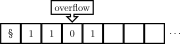
\includegraphics{res/turing_add1_4}
  \caption{A Turing machine}
  \label{fig:Turing machine}
\end{figure}

\begin{defin}
  Let $\mathbb A = (S, δ)$ be a Turing machine. A \emph{configuration}
  of $\mathbb A$ is a triple $(s, j, c) ∈ S × ℕ × A^ℕ$. It reflects
  the current state of $\mathbb A$, the current position of its
  head, and the content of its work-tape.
\end{defin}

A configuration of the form $(\shalt, 0, c)$ is called \emph{halting}. A
\emph{start configuration} is of the form $(\sstart, 0, c)$ such that $c(0) =
\sta$ and there exists an $n ∈ ℕ$ such that $c(i) = \emp$ if and only if $i >
n$. This means that in a start configuration the work-tape reads
\[
  \sta x_1 x_2 … x_n \emp \emp …
\]
It will be very convenient to identify the finite string $x_1…x_n$ with this
tape content.

\begin{defin}
  One writes $(s, j, c) \vdash_1 (s', j', c')$ and calls $(s', j', c')$ a
  \emph{successor configuration} of $(s, j, c)$ if there exists an $m ∈ \lbrace
  -1, 0, 1 \rbrace$ such that

  \begin{itemize}
  \item
    $δ(s, c) = (s', c', m)$,
  \item
    $j' = j + m$, and
  \item
    $c'(ℓ) = c(ℓ)$ for all $ℓ ≠ j$.
  \end{itemize}

  This relation makes the set of all configurations of $\mathbb A$ into a
  directed graph. A \emph{run} of $\mathbb A$ on $x$ is a path in this directed
  graph starting at the start configuration $(\sstart, 0, x)$. A run of
  $\mathbb A$ on $x$ is \emph{halting} or \emph{complete} if it reaches a
  halting configuration $(\shalt, 0, y)$. In this case I write $\mathbb A (x) =
  y$.
\end{defin}

I will denote Turing machines using listings, where the fact that
$δ_\text{delta} (\state{state}, b) = (\state{state'}, c, m)$ is encoded by

\begin{lstlisting}
delta "state" c = ("state'", c', m)
\end{lstlisting}

Variables \verb+c+ match all possible states or characters in the alphabet
respectively. However, I follow the convention that if an assignment of
variables matches more than one pattern, the first matching pattern is chosen.
This means that
%
\begin{lstlisting}
delta "state" 1 = ("state'", 1, 1)
delta "state" c = ("state''", c, 0)
\end{lstlisting}
%
should be interpreted as
%
\[ δ(s, c) =
  \begin{cases}
    (\state{state'}, \one, 1) & \text{if } s=\state{state} ∧ c = \one\\
    (\state{state''}, c, 0) & \text{if } s=\state{state} ∧ c ≠ \one
  \end{cases}.
\]

See \cref{app:turing} on how to simulate Turing machines
using the \emph{Haskell} programming language.

\begin{exam}
    Consider the Turing machine $\mathbb A_\text{add1} = (\lbrace \sstart,
    \shalt, \state{overflow}, \state{return}, \state{error} \rbrace,
    δ_\text{add1})$ that adds $1$ to a (possibly zero-patched) binary
    representation of a natural number $n$. Its transition function is described
    in \cref{lst:add1}. The last line of the program ensures, that $δ$ is a
    total function, as it matches all remaining pairs of states and
    characters and lets the machine enter the state $\state{error}$. The
    complete run of $\mathbb A_\text{add1}$ on $\one\one\zer\one$ can be seen in
    \cref{fig:complete run}.
\end{exam}

\lstinputlisting[float, frame=tb,
                 caption=A Turing machine adding one to the input string,
                 label=lst:add1]{./listings/add1.hs}

\begin{figure*}
    \begin{subfigure}{.5\textwidth}
        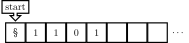
\includegraphics{res/turing_add1_1}
        \caption{$δ(\sstart, \sta) = (s_\text{overflow}, \sta, 1)$}
    \end{subfigure}

    \begin{subfigure}{.5\textwidth}
        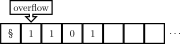
\includegraphics{res/turing_add1_2}
        \caption{$δ(s_\text{overflow}, \one) = (s_\text{overflow}, \one, 1)$}
    \end{subfigure}

    \begin{subfigure}{.5\textwidth}
        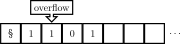
\includegraphics{res/turing_add1_3}
        \caption{$δ(s_\text{overflow}, \one) = (s_\text{overflow}, \one, 1)$}
    \end{subfigure}

    \begin{subfigure}{.5\textwidth}
        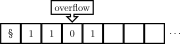
\includegraphics{res/turing_add1_4}
        \caption{$δ(s_\text{overflow}, \zer) = (s_\text{return}, \one, -1)$}
    \end{subfigure}

    \begin{subfigure}{.5\textwidth}
        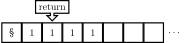
\includegraphics{res/turing_add1_5}
        \caption{$δ(s_\text{return}, \one) = (s_\text{return}, \one, -1)$}
    \end{subfigure}

    \begin{subfigure}{.5\textwidth}
        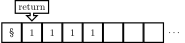
\includegraphics{res/turing_add1_6}
        \caption{$δ(s_\text{return}, \one) = (s_\text{return}, \one, -1)$}
    \end{subfigure}

    \begin{subfigure}{.5\textwidth}
        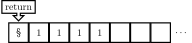
\includegraphics{res/turing_add1_7}
        \caption{$δ(s_\text{return}, \sta) = (s_\text{halt}, \sta, 0)$}
    \end{subfigure}

    \begin{subfigure}{.5\textwidth}
        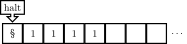
\includegraphics{res/turing_add1_8}
        \caption{$δ(s_\text{halt}, \sta) = (s_\text{halt}, \sta, 0)$}
    \end{subfigure}

    \caption{The complete run of $\mathbb A_\text{add1}$ on $\one\one\zer\one$}
    \label{fig:complete run}
\end{figure*}

\begin{defin}
    Let $\mathbb A$ be a Turing machine.

    \begin{thmlist}
        \item
          $\mathbb A$ \emph{computes} the partial function that maps each
          $x$ with a complete run to $\mathbb A(x)$ and is undefined for all
          other strings.
        \item
          $\mathbb A$ \emph{accepts} all $x$ such that
          $\mathbb A(x) = \one$ and \emph{rejects} them if
          $\mathbb A(x) = \zer$.
        \item
          A partial function on $\lbrace \zer, \one \rbrace^*$ is
          \emph{computable} if there is a Turing machine computing it. Sometimes
          computable functions are referred to as \emph{recursive} or
          \emph{efficient} functions.
        \item
          A subset of $\lbrace \zer, \one \rbrace^*$, i.e. a
          problem, is \emph{decidable} if there is a Turing machine computing
          its characteristic function.
        \item
          A problem is called \emph{semi-decidable} or \emph{computably
          enumerable} if there is a Turing machine accepting precisely the
          elements of the problem.
    \end{thmlist}
\end{defin}

The last item of the definition above means that a problem is
semi-decidable if there is a Turing machine affirming membership of the
corresponding set but it might not be able to refute membership.

Note that every finite problem is decidable by a Turing machine that reads the
tape content and checks at every step whether there are elements in the problem
that start with the tape content the machine has read. After $n + 1$ steps,
where $n$ denotes the length of the longest string in the problem, the machine
stops at the latest.

\begin{lem} \label{lem:composition of Turing machines}
  Let $\mathbb A_1 = (S_1, δ_1)$ and $\mathbb A_2 = (S_2, δ_2)$ be Turing
  machines computing $f_1: D_1 → \set{\zer, \one}^*$ and $f_2: D_2 → \set{\zer,
  \one}^*$ respectively ($D_1, D_2 \subseteq \set{\zer, \one}^*$). Then there
  exists a Turing machine $\mathbb A_{f_2 \circ f_1}$ computing the partial
  function $f_2 \circ f_1: D_1 ∩ f_1^{-1}(D_2) → \set{\zer, \one}^*$ obtained by
  composing $f_1$ and $f_2$.
\end{lem}
\begin{proof}
  One constructs $\mathbb A_{f_2 \circ f_1}$ from $\mathbb A_1$ and $\mathbb
  A_2$ as follows. Let $S_1 = \set{\sstart, \shalt} \sqcup S_1'$ and $S_2 =
  \set{\sstart, \shalt} \sqcup S_2'$, then set $S = \set{\sstart, \shalt} \sqcup
  S_1' \sqcup S_2' \sqcup \set{\state{compose}}$, where $\sqcup$ denotes the
  disjoint union. Now set for $c ∈ A$
  %
  \begin{align*}
    δ (s, c) &=
      \begin{cases}
        δ_1 (s, c) & \text{if } s ∈ S_1' ∪ \set\sstart \\
        (\state{compose}, c', m) & \text{if } s ∈ S_1 \text{ and } δ_1(s, c) = (\shalt, c', m)\\
        δ_2 (s, c) & \text{if } s ∈ S_2' ∪ \set\shalt \\
      \end{cases}, \\
    δ (\state{compose}, c) &= δ_2 (\sstart, c).
  \end{align*}
  %
  Then $\mathbb A_{f_2 \circ f_1} = (S, δ)$ computes $f_1 \circ f_2$ because $δ$
  is defined to first run the program of $\mathbb A_1$ and if this machine would
  reach a halting state run $\mathbb A_2$.
\end{proof}
% IDEA Maybe: A semi-decidable set is decidable iff its complement is semi-decidable
\todo{Maybe: A semi-decidable set is decidable iff its complement is semi-decidable}

\begin{exam}
    One can encode a natural number $n$

    \begin{exlist}
    \item \label{ex:tally encoding}
      in tally notation
      \begin{align*}
        n & ↦ \underbrace{\one…\one}_{n\text{-times}}, \quad \text{if } n > 0 \\
        0 & ↦ λ
      \end{align*}
    \item
      by its binary representation
      \begin{align*}
          n = 2^k + \sum_{i = 0}^{k-1} b_i 2^i & ↦ b_0…b_{k-1}\one, \quad
              \text{if } n > 0\\
                                             0 & ↦ \zer,
      \end{align*}
      or
    \item \label{ex:omega encoding}
      by a shifted and truncated form of its binary representation
      \begin{align*}
        n = 1 + \sum_{i = 0}^k b_i 2^i & ↦ b_0…b_k, \quad \text{if } n > 0\\
                                     0 & ↦ λ
      \end{align*}

      In other words, $n$ is mapped to the $n$-th string if one orders $\lbrace
      \zer, \one \rbrace ^ ℕ$ lexicographically. Following a tradition in
      logics I denote $ℕ$ under this last encoding by $ω$.
    \end{exlist}

    In either case the set obtained by encoding $ℕ$ is easily seen to be
    decidable. In the first case, check that the string contains only copies
    of the bit $\one$. Indeed, this can be achieved by the Turing machine
    %
    \[\mathbb A_\text{tally} =
      ( \lbrace \sstart, \shalt, \scheck, \state{accept}, \state{reject},
        \state{rejectMR}, \state{error} \rbrace, δ),\]
    %
    whose transition function is displayed in \cref{lst:tally encoding}.

    In the second case it suffices to check that the string has length $1$
    or ends in an $\one$, and in the third case every string is accepted.
\end{exam}

\lstinputlisting[float, frame=tb,
                 caption=A Turing machine checking whether the input is tally-encoded,
                 label=lst:tally encoding]{./listings/tally.hs}

Taking another look at the definition of computability, one sees that only unary
functions defined on subsets of $ω$, mapping to subsets of $ω$ can be
computable. However, one can easily extend this to functions on multiple
variables, by encoding tuples in $ω \times ω$ by elements of $ω$ in such a way,
that the projections $p_i: \enc{(x_1, x_2)} ↦ x_i$  for $i ∈ \lbrace 0, 1
\rbrace$ are uniformly computable. This means, there are injective pairing
functions $ω^2 → ω$ and Turing machines $\mathbb P_1, \mathbb P_2$
computing $p_1$ or $p_2$ respectively. Clearly if one has a pairing function $ℕ^2 → ℕ$ then one immediately obtains a pairing function $ω^2 → ω$
by composing with the encoding function.

\begin{exam}[Pairing functions]
  \begin{exlist}
    \item\label{ex:tally pairing}
    Using tally notation on can encode $(n, m) ∈ ℕ^2$ by
    \[
      ⟨\enc{n}, \enc{m}⟩ = \underbrace{\one … \one}_{n\text{-times}} \zer \underbrace{\one … \one}_{m\text{-times}}
    \]

    \item A simple pairing function encodes the pair $(b_1b_2…b_n, c_1c_2…c_m) ∈ ω^2$

    \[ ⟨b_1b_2…b_n, c_1c_2…c_m⟩ = b_1b_1b_2b_2…b_nb_n \zer\one c_1c_2…c_m. \]
  \end{exlist}
\end{exam}

Of course by applying a pairing function iteratively one obtains an $n$-ary pairing function. The projections need to be composed accordingly. For example
\[
  (x_1, x_2, x_3) ↦ ⟨x_1, ⟨x_2, x_3⟩⟩
\]
yields a ternary pairing function and $π_1\circ π_2$ is the projection onto
$x_2$. Using any of the pairing functions above, one can consider $n$-ary
computable functions by providing the encoded pair $⟨x_1, x_2, …, x_n⟩$ as the
single argument of a Turing machine $\mathbb A$. If the context is clear, I will
write $\mathbb A(\seq{x})$ in this situation.

In the remainder of this thesis I will make use of the following
meta-mathematical thesis. That cannot be mathematically proven but has been
heuristically justified for all of the generally accepted\footnote{The
interested reader should find the comment \cite{Davis2006} on hyper-computation
by Davis quite revealing.} formalisations of computation. It allows one to state
properties of computation without referring to a specific model.

\begin{churchturing}
  The class of intuitively computable
  functions coincides with the class of all Turing computable functions.
\end{churchturing}

One of the fundamental theorems of theoretical computer science is the
existence of a universal Turing machine.

\begin{thm}
    There exists a Turing machine $\mathbb U$ that computes upon receiving
    the tuple $(\ulcorner \mathbb A \urcorner, x)$ as input, the output of
    Turing machine $\mathbb A$ on $x$ i.e.
    \[ \mathbb U(\ulcorner \mathbb A \urcorner, x) = y \Leftrightarrow \mathbb A (x) = y\]
\end{thm}

A natural question is:

\begin{quote}
  Given a machine $\mathbb A$ and a string $x$. Does $\mathbb A$
  halt on $x$?
\end{quote}

It is one of the most fundamental results of theoretical computer science that
the halting problem is undecidable. The contradiction to the existence of a
Turing machine deciding this problem is obtained by a diagonalisation technique
that is also present in Cantor's proof that the power set of the integers is
uncountable or Russel's paradox. However, the idea is best encapsulated by the
illustration of Carlo Chiostri, based on Carlo Collodi's fairy tale novel ‘The
Adventures of Pinocchio’, displayed in \cref{fig:Pinocchio}.

\begin{figure}
  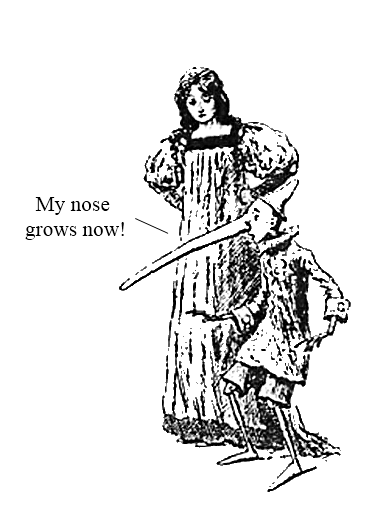
\includegraphics[height=30ex]{res/Pinocchio_paradox.png}
  \caption{Pinocchio says a lie and stretches his nose}
  \label{fig:Pinocchio}
\end{figure}

\begin{thm}
    The halting problem is undecidable.
\end{thm}
\begin{proof}
    Assume there exists a Turing machine $\mathbb B$ that decides the
    halting problem i.e.~for all Turing machines $\mathbb A$ and all
    strings $x$

    \[ \mathbb B(\enc{\mathbb A}, x) =
    \begin{cases}
      \one  & \text{if } \mathbb A \text{ halts on } x\\
      \zer  & \text{if } \mathbb A \text{ does not halt on } x
    \end{cases}\]

    Now using $\mathbb B$ construct a Turing machine $\mathbb B'$ that
    simulates $\mathbb B(\enc{\mathbb A}, \enc{\mathbb A})$ on its input
    $\enc{\mathbb A}$ and enters an infinite loop if
    $\mathbb B(\enc{\mathbb A}, \enc{\mathbb A}) = \zer$. Expressed more
    formally this means

    \[
      \mathbb B' \text{ halts on } \enc{\mathbb A} ⇔
      \mathbb A \text{ does not halts on } \enc{\mathbb A}.
    \]

    Setting $\mathbb A = \mathbb B'$ yields the desired contradiction.
\end{proof}

For a more detailed proof of this fact and lot more information on computability
see \cite{Cooper2004}. As the halting problem is undecidable the halting set
defined by
\[
 \mathcal{K} = \set{⟨\enc{\mathbb A}, x⟩ \mid \mathbb A \text{ halts on } x}
\]
is undecidable. However using the universal Turing machine it is clearly
semi-decidable.


\section{Prerequisites from number theory}
% !TeX encoding = UTF-8
% !TeX TS-program = xelatex
% !TeX spellcheck = en_GB
% !TeX root = ../Herbstrith-H10_over_AI.tex
% TODO
\todo{Fill out these theorems and definitions}

\subsection{Definitions}

\begin{defin}[class number $c_k$]
    pass
\end{defin}

\begin{defin}[Abelian extension]
    pass
\end{defin}

\subsection{Theorems}

Let $V$ be an $n$-dimensional vector space over the reals $ℝ$. If $\seq[k]{e} ∈
V$ ($k ≤ n$) are linearly independent over $ℝ$, then the free Abelian group
\[
  Λ = ℤ e_1 + … + ℤ e_k
\]
is called a \emph{lattice}. Note that $ℤ + \sqrt{2} ℤ$ is not a lattice in this
sense, because $1$ and $\sqrt{2}$ are linearly dependent over $ℝ$.

Let $μ$ be the measure corresponding to the usual Euclidean volume%
\footnote{I.e. $μ$ is the Lebesgue measure on $ℝ^n$ and therefore the Haar
measure with respect to the locally compact, Abelian group $⟨Λ, +⟩$.}
on $ℝ^n$. Then the \emph{fundamental parallelepiped}
\[
  D = \set{\sum_{i=1}^n α_i e_i \;\middle\vert\; α_i ∈ [0, 1]}
\]
has the volume
\[
  μ(D) = |\det \left( \seq{e} \right)|
\]
for a fixed lattice $Λ = ℤ e_1 + … + ℤ e_n$ in $ℝ^n$. One calls such a lattice whose rank coincides with the dimension of the vector space $ℝ^n$ a \emph{full} lattice.

\begin{thm}[Minkowski's theorem] \label{thm:Minkowski}
  Let $Λ = ℤ e_1 + … + ℤ e_n$ be a full lattice in the $n$-dimensional $ℝ$-vector space $V$ and let $D$ denote its fundamental parallelepiped. If $T \subseteq V$ is compact, convex and symmetric in the origin, i.e. if $α ∈ T$ so is $-α ∈ T$, and
  \[
    μ(T) ≥ 2^n μ(D).
  \]
  Then $T$ contains a non-zero lattice point $α ∈ Λ \setminus \set{0}$.
\end{thm}

For a proof of Minkowski's theorem and further details on lattices see \cite[4.4, p.~28, German]{Neukirch2006} or \cite[Thm.~4.19]{Milne2017}.

\begin{thm}[Dirichlet's unit theorem]
    see \cite[Thm.~5.1]{Milne2017}
\end{thm}

\begin{thm}[Local-Global--Principle / Hasse-Minkowski theorem]
    see \cite[§ 66]{Meara2000}
\end{thm}


\chapter{Hilbert's tenth problem}

\section{Different perspectives on an old problem}
% !TEX encoding = UTF-8
% !TEX TS-program = xelatex
% !TEX spellcheck = en_GB
% !TEX engine = xelatex
% !TEX root = ../Herbstrith-H10_over_AI.tex
%
% ##     ##    ##     #####      ##     ## ####  ######  ########
% ##     ##  ####    ##   ##     ##     ##  ##  ##    ##    ##
% ##     ##    ##   ##     ##    ##     ##  ##  ##          ##
% #########    ##   ##     ##    #########  ##   ######     ##
% ##     ##    ##   ##     ##    ##     ##  ##        ##    ##
% ##     ##    ##    ##   ##     ##     ##  ##  ##    ##    ##    ###
% ##     ##  ######   #####      ##     ## ####  ######     ##    ###

\subsection{Diophantine equations and sets}
%   ##
% ####
%   ##
%   ##
%   ##
%   ##
% ######

In 1900, David Hilbert held his famous lecture~\cite{Hilbert1900} before the
\emph{Second International Congress of Mathematicians} in Paris. The lecture
entitled \foreignquote{german}{Mathematische Probleme} contained 23
mathematical problems left for the 20th century to solve. The tenth of these
problems and its variants are the subject of this thesis. The problem states

\begin{foreigndisplayquote}{german}
  \textsc{10. Entscheidung der Lösbarkeit einer Diophantischen Gleichung.}
  Eine Diophantische Gleichung mit irgend welchen Unbekannten und mit
  ganzen rationalen Zahlencoefficienten sei vorgelegt: man soll ein Verfahren
  angeben, nach welchem sich mittelst einer endlichen Anzahl von Operationen
  entscheiden läßt, ob die Gleichung in ganzen rationalen Zahlen lösbar ist.%
  \footnote{
    \begin{english}
      \textsc{10. Determination of the solvability of a diophantine equation.}
      Given a diophantine equation with any number of unknown quantities and
      with rational integral numerical coefficients: To devise a process
      according to which it can be determined by a finite number of operations
      whether the equation is solvable in rational integers.
      \hspace*{\fill}\cite[translation published in][]{Hilbert2000}
    \end{english}
  }
  \hspace*{\fill}\cite{Hilbert1900}
\end{foreigndisplayquote}

A \emph{Diophantine equation}---in the classical sense---is of the form
\[
  p(α_1, …, α_n) = 0,
\]
where $p ∈ ℤ[X_1, …, X_n]$ is a polynomial and one only allows rational integral
solutions $α_1,…,α_n ∈ ℤ$. Using the tools developed in \cref{sec:model
theory,sec:number theory}, we will exchange one or both occurrences of the
rational integers by values from other rings. It took until the 1930s to
formalize what Hilbert meant by a \foreignquote{german}{Verfahren \textins{mit}
einer endlichen Anzahl von Operationen%
\footnote{\foreignquote{english}{%
  process \textins{with} a finite number of operations}
}}
to the notion of \emph{computation} that was defined in \cref{sec:computability
theory}. In the same section we have also defined what it means to \emph{decide
a problem}, so we are left with the task of identifying Hilbert's question with
a set of strings. In a first approach one could reformulate the tenth problem as
\begin{quote}
  For a fixed polynomial \(p ∈ ℤ[X_1, X_2, …]\) does there exist a Turing
  machine \(\mathbb{A}_p\) that returns \(\one\) if \(p\) has a root and
  \(\zer\) otherwise?
\end{quote}
This formalization is however trivially solvable, as the Turing machine in
question takes no input and thus must always return either \(\one\) or \(\zer\).
But such machines returning a constant value are easily constructable. We must
therefore exchange the quantifiers and ask
\begin{quote}
  Does there exist a Turing machine \(\mathbb{A}\) and an encoding
  \(\enc{\cdot}\) such that for all polynomials \(p ∈ ℤ[X_1, X_2, …]\) the
  output \(\mathbb{A}(\enc{p})\) is \(\one\), if \(p\) has integral roots, and
  \(\zer\) otherwise.
\end{quote}

We will see that if we restrict ourselves to encodings \(\enc{\cdot}\) that
allow to efficiently obtain the evaluation \(\enc{p(\mathbf{α})}\) from
\(\enc{p}\) and \(\enc{\mathbf{α}}\), then the answer to the question above is
negative. In fact, for all rings of algebraic integers \(\algint\), that we will
consider, we will find a single multivariate polynomial \(p_{\mathcal{K}}(X,
\seq{Y}) ∈ \algint[X, \seq{Y}]\) such that for all Turing machines
\(\mathbb{A}\) there exists an algebraic integer \(α ∈ \algint\) with the
property that \(\mathbb{A}\) cannot correctly decide whether the partially
evaluated polynomial
\[
  p_{\mathcal{K}}(α, \seq{Y})
\]
has roots in \(\algint\). The index \(\mathcal{K}\) of the polynomial above is
not chosen at random. Indeed, the polynomial \(p_{\mathcal{K}}\) represents an
encoded version of the halting set \(\mathcal{K}\) in the following sense:

\begin{defin}
    Let $R$ be a commutative ring with one. A set $S \subseteq R^n$ is said to
    be \emph{Diophantine} over \(R\) if there exists a polynomial $p ∈
    R[X_1,…,X_n, Y_1,…,Y_m]$ in \(n + m\) many indeterminates (\(m,n ≥ 0\)) such
    that
    \[
      (α_1,…,α_n) ∈ S ⇔
      ∃ β_1,…,β_m ∈ R: p(α_1,…,α_n,β_1,…,β_m) = 0
    \]
\end{defin}

A polynomial $p ∈ R[X_1, …, X_n]$ as above defines an $n$-ary relation $\rel{p}$
on \(R\) by
\[
  \rel{p}(α_1, …, α_n)  \quad :⇔ \quad p(α_1, …, α_n) = 0
\]
In this sense a set $S \subseteq R^i$ is Diophantine if there exists a
polynomial $p ∈ R[X_1, …, X_n]$ such that
\[
  (\seq[i]{α}) ∈ S \quad ⇔ \quad
  ∃ \seq[n - i]{β} : \rel{p}(\seq[i]{α}, \seq[n - i]{β})
\]

Viewing $n$-ary relations as subsets of $R^n$, I will sometimes refer to
Diophantine sets as \emph{Diophantine relations}. A function $R^n → R^m$ is
called \emph{Diophantine} if it is Diophantine viewed as an \((n + m)\)-ary
relation.

\begin{exam}\label{ex:Diophantine sets}
  \begin{exlist}
    \item Let $R$ be an integral domain.
    Then every finite subset $S$ of $R$ is Diophantine, because the roots of
    \[
      p(X) := \prod_{s ∈ S} (X - s)
    \]
    are precisely the elements of $S$.

    \item Let \(R\) be an integral domain. Then for every polynomial \(p ∈
    R[X_1, …, X_n]\) the associated polynomial function \(p: R^n → R\) is
    Diophantine. To see this we set
    \[
      q(X_1, …, X_n, X_{n + 1}) := p(\seq{X}) - X_{n + 1},
    \]
    and notice that \(q\) has a root \((\seq{α}, α_{n + 1}) ∈ R\) if and only if
    \(p(\seq{α}) = α_{n + 1}\) as claimed.

    \item Let $R$ be a commutative ring with unit. Then divisibility in $R$ is
    Diophantine. Indeed $α_1 \mid α_2$ in $R$ precisely if
    \[
      ∃ β ∈ R : α_1 β = α_2.
    \]

    \item Let $K$ be a number field and $\algint$ its ring of algebraic integers. Then $\algint \setminus \set{0}$ is
    Diophantine over $\algint$. I extend the hint stated in \cite[Prop. 1]{Denef1978} and claim that
    \[
      α ≠ 0 ⇔ ∃ β, γ ∈ \algint : α β = (2 γ - 1)(3 γ - 1).
    \]

    Firstly, note that the polynomial on the right hand side has the roots $1/2$
    and $1/3$ in $ℚ$. As the intersection $\algint ∩ ℚ $ equals $ℤ$ for all
    number fields $K$, one obtains that the polynomial identity can only be
    satisfied for $α ≠ 0$.

    Let now \(α ≠ 0\). We can decompose the ideal \((α) = \mathfrak x_2
    \mathfrak x_3\) such that
    \[
    (2) + \mathfrak x_2 =
    \algint, \; (3) + \mathfrak x_3 = \algint \, \text{and } \, \mathfrak x_2 +
    \mathfrak x_3 = \algint.
    \]
    This is because \(2\) and \(3\) are rational primes and therefore \((2)\)
    and \((3)\) are relative prime.
    % see Baxa Thm 120
    In other words, we find
    \[
      ∃ x_2 ∈ \mathfrak x_2, ∃ y_2 ∈ \algint : 2 y_2 + x_2 = 1 \quad \text{and} \quad
      ∃ x_3 ∈ \mathfrak x_3, ∃ y_3 ∈ \algint : 3 y_3 + x_3 = 1
    \]
     As a consequence of the Chinese remainder theorem (\cref{thm:Chinese
     remainder}) the congruences
    \[
      γ \equiv y_2 \mod \mathfrak x_2 \quad \text{and} \quad
      γ \equiv y_3 \mod \mathfrak x_3
    \]
    are simultaneously solvable. This implies that
    \[
      2 γ \equiv 2 y_2 \equiv 1 \mod \mathfrak x_2 \quad \text{and} \quad
      3 γ \equiv 3 y_3 \equiv 1 \mod \mathfrak x_3.
    \]
    Which can be rewritten as
    \[
      2 γ - 1 ∈ \mathfrak x_2  \quad \text{and} \quad
      3 γ - 1 ∈ \mathfrak x_3.
    \]
    As a consequence, \((2 γ - 1)(3 γ - 1)\) is contained in \(\mathfrak x_2
    \mathfrak x_3 = (α)\), or put differently, there exists a \(β ∈ \algint\)
    such that
    \[
      α β = (2 γ - 1)(3 γ - 1).
    \]

    \item\label{ex:U K is Diophantine}
    Let \(R\) be a commutative ring with unit. The set of units \(U\) in \(R\) is Diophantine over \(R\). This can be seen by the polynomial equation
    \[
      x ∈ U \quad ⇔ \quad ∃ y : xy = 1.
    \]
  \end{exlist}
\end{exam}

In the examples above we have seen that many sets and relations are Diophantine.
Before we go on proving some structural results for Diophantine sets, we turn
our attention to the classical case of Diophantine subsets of \(ℤ\) and study
their relations with subsets of \(ℕ\).

\begin{exam}[Diophantine subsets of \(ℕ\)]\label{ex:N is Diophantine over Z}
  If one wants to study sets that are Diophantine over \(ℕ\), one runs into the
  problem that \(ℕ\) is not a ring. An approach that has been carried out
  \cite[cf.~e.g.][]{Davis1973} is considering sets \(S ⊂ ℤ^n\) that are
  Diophantine over \(ℤ\) and intersecting them with \(ℕ^n\). I will show that
  this construction can be carried out in a Diophantine way.

  First, we note that if \(S_1, S_2 ∈ ℤ^n\) are Diophantine over \(ℤ\), then
  their intersection is Diophantine over \(ℤ\) as well. This is because if
  \(p_1 ∈ ℤ[\seq{X}, \seq[m_1]{Y}]\) represents \(S_1\) via
  \[
    (\seq{α}) ∈ S_1 \quad ⇔ \quad
    ∃ \seq[m_1]{β} : p_1(\seq{α}, \seq[m_1]{β}) = 0
  \]
  and \(p_2 ∈ ℤ[\seq{X}, \seq[m_1]{Y}]\) represents \(S_2\), we set \(m := m_1 +
  m_2\) and consider \(p_1\) and \(p_2\) as polynomials in \(n + m\) many
  indeterminates, where for all \(i ∈ \set{n + 1, …, m}\) indeterminate \(Y_i\)
  either appears in \(p_1\) or \(p_2\) but not in both. Then \((\seq{α},
  \seq[m]{β}) ∈ ℤ^{m + n}\) is a root of
  \[
    q(\seq{X}, \seq[m]{Y}) :=
      p_1(\seq{X}, \seq[m]{Y})^2 + p_2(\seq{X}, \seq[m]{Y})^2
  \]
  if and only if \((\seq{α}, \seq[m]{β})\) is a root of \(p_1\) and \(p_2\).
  Thus, we find that
  \[
    S_1 ∩ S_2 =
    \set{\seq{α} ∈ ℤ \mid ∃ \seq[m]{β} ∈ ℤ : q(\seq{α}, \seq[m]{β}) = 0}.
  \]

  By Lagrange's four square-theorem (\cref{cor:Lagranges four square theorem})
  we know that every non-negative integer \(α\) is the sum of four squares and
  as a consequence
  \[
    x ∈ ℕ \quad ⇔ \quad
    ∃β_1,β_2,β_3,β_4∈ℤ: β_1^2 + β_2^2 + β_3^2 + β_4^2 = α.
  \]
  is a Diophantine definition of $ℕ$ over $ℤ$. Therefore, we can check for a
  given polynomial equation whether all variables take only non-negative values
  in a Diophantine way. More formally, we say that  a subset \(S ⊂ ℕ^n\) is
  \emph{Diophantine over \(ℕ\)} if there exists a polynomial \(p ∈ ℤ[X_1, …,
  X_n, Y_1, …, Y_m]\) such that
  \[
    (\seq{α}) ∈ S \quad ⇔ \quad
    ∃ \seq[m]{β} ∈ ℕ : p(\seq{α}, \seq[m]{β}) = 0.
  \]
  If this is the case, we find that \(S\) is Diophantine over \(ℤ\) as well, by
  conjugating the identity with the clause
  \[
    \left(\bigwedge_{i = 1}^n ∃ γ_{i1}, …, γ_{i4} ∈ ℤ :
      α_i = \sum_{j = 1}^4 γ_{ij}^2 \right) ∧
    \left(\bigwedge_{i = 1}^m ∃ δ_{i1}, …, δ_{i4} ∈ ℤ :
      β_i = \sum_{j = 1}^4 δ_{ij}^2 \right).
  \]

  We now list some examples of sets that are Diophantine over \(ℕ\).
  \begin{exlist}
    \item The set of composite numbers is Diophantine over $ℕ$, as $α ∈ ℕ$ is
    composite if and only if
    \[
      ∃ β_1, β_2 ∈ ℕ : x = (β_1 + 2) (β_2 + 2).
    \]
    Here adding $2$ to $β_1$ and $β_2$ ensures, that both factors are greater
    than $1$. Choosing
    \[
      p(X, Y_1, Y_2) := X - (Y_1 + 2)(Y_2 + 2)
    \]
    yields the claim. To transform this into a Diophantine definition over
    \(ℤ\), we must conjugate the clauses stating that \(α, β_1\) and \(β_2\) are
    non-negative. Thus, we obtain
    \begin{align*}
      ∃ β_1, β_2, γ_1, …, γ_4, δ_{11}, …, δ_{14}, δ_{21}, …, δ_{24} ∈ ℤ: (
        & x = (β_1 + 2) (β_2 + 2) ∧\\
        & x = γ_1^2 + γ_2^2 + γ_3^2 + γ_4^2 ∧\\
        & β_1 = (δ_{11}^2 + δ_{12}^2 + δ_{13}^2 + δ_{14}^2 ∧\\
        & β_2 = (δ_{21}^2 + δ_{22}^2 + δ_{23}^2 + δ_{24}^2),
    \end{align*}
    which can be rewritten as the single Diophantine identity
    \begin{align*}
      ∃ β_1, β_2, & γ_1, …, γ_4, δ_{11}, …, δ_{14}, δ_{21}, …, δ_{24} ∈ ℤ:\\
        & \left(\left(\left(x - (β_1 + 2) (β_2 + 2)\right)^2 +
          \left(x - (γ_1^2 + γ_2^2 + γ_3^2 + γ_4^2)\right)^2\right)^2 +\right.\\
        & \left. +
          \left(
            β_1 - (δ_{11}^2 + δ_{12}^2 + δ_{13}^2 + δ_{14}^2)\right)^2
          \right)^2 +
          \left(β_2 - (δ_{21}^2 + δ_{22}^2 + δ_{23}^2 + δ_{24}^2)\right)^2.
    \end{align*}

    \item The usual order relation $≤$ on $ℕ$ is Diophantine over $ℕ$.
    Indeed $α_1 ≤ α_2$ in $ℕ$ if and only if
    \[
      ∃ β ∈ ℕ : α_1 + β  = α_2.
    \]
  \end{exlist}
\end{exam}

We will now see how one can describe Diophantine sets from the view of model
theory.

\begin{lem}
  Let \(R\) be a commutative ring with one and let \(\mathfrak{R}\) be its
  \(\lang_{ring}\)-structure. Then \(S ⊂ R^n\) is Diophantine if and only if
  there exists an atomic \(\lang_R\)-formula \(ϕ(\mathtt{\seq{x}, \seq[m]{y}})\)
  such that
  \[
    (\seq{α}) ∈ S \quad ⇔ \quad
    \mathfrak{R} \models \mathtt{∃ y_1 : … ∃ y_m: }
        ϕ(\seq{α}, \mathtt{\seq[m]{y}})
  \]
  holds.
\end{lem}
\begin{proof}
  By \cref{thm:Diophantine theory} the forumla \(ϕ(\seq{α}, \seq[m]{β})\) is
  true in \(\mathfrak{R}\) if and only if the polynomial associated with \(ϕ\)
  has a root in \((\seq{α}, \seq[m]{β})\).
\end{proof}

Note that even more is true as a partially evaluated polynomial is still a
polynomial. Thus, one can decide membership in all Diophantine sets if and only
if one can decide for all polynomials whether they have roots. Thus, if \(R\) is
a countable commutative ring with one, we can identify Hilbert's tenth problem
over \(R\) with the set of Gödel numbers of \(\mathtt{H10}(\mathfrak{R})\).

\begin{lem}\label{lem:intersections and unions}
    Let $R$ be an integral domain, whose quotient field $\Quot R$ is not
    algebraically closed. Then if $S_1, S_2 \subseteq R$ are Diophantine so are
    \[
      S_1 ∩ S_2 \quad \text{and} \quad S_1 ∪ S_2.
    \]

    If $R$ is computable, then there is an algorithm that derives the defining
    polynomial equations for union and intersection efficiently from the
    equations of $S_1$ and $S_2$.
\end{lem}

In other words, conjunctions and disjunctions of existentially quantified atomic
formulae can be replaced by a single existentially quantified atomic formula. Or
again put differently, conjunction $∧$ and disjunction $∨$ are
$\lang_{ring}$-definable, efficiently computable predicates.

\begin{proof}
  Let \(p(\seq{X}, \seq[m_1]{Y})\) and \(q(\seq{X}, \seq[m_2]{Y})\) give
  Diophantine definitions of $S_1$ and $S_2$ resp. Then as in \cref{ex:N is
  Diophantine over Z} we set \(m = m_1 + m_2\) and interpret \(p, q\) as
  polynomials in \(n + m\) many indeterminates such that for all \(i ∈ \set{n +
  1, …, m}\) indeterminate \(Y_i\) appears either in \(p\) or \(q\) but not
  in both.

  Now set
  \[
    h := p q.
  \]
  Then \(h\) vanishes if and only if $p$ or $q$ vanishes. As a consequence, the
  \(n\)-tuple \(\seq{α} ∈ R\) is in the union of \(S_1\) and \(S_2\) if and only
  if
  \[
    ∃ \seq[m]{β} ∈ R : h(\seq{α}, \seq[m]{β}) = 0.
  \]

  To make notation easier when proving the claim for intersections, I will
  assume that \(n = 1\) and \(m = 2\). The general cases follows completely
  analogously. Now let
  \[
    h(T) = a_k T^k + … + a_1 T + a_0 ∈ R[T]
  \]
  be a polynomial of degree $k > 0$ without roots in $\Quot R$. Then $\overline
  h(T) = T^k h(T^{-1})$ does not have roots in $\Quot R$ either. As if $α ∈
  \Quot R$ is a root of $\overline h$ then
  \[
    0 = \overline h(α) = a_k + a_{k-1} α + a_1 α^{-1} + a_0 α^k
  \]
  and $α = 0$ implies that $a_k = 0$. Otherwise, $α^{-1}$ is a root of
  $α^k h$ and therefore of $h$.

  Now consider
  \[
    H(α, β_1, β_2) =
    \sum_{i=0}^k a_i p(α, β_1)^i q(α, β_2)^{k - i}.
  \]
  I will prove for all $α, β_1, β_2 ∈ R$ that \(H(α, β_1, β_2) = 0\) precisely
  if \(p(α, β_1)\) and \(p(α, β_2)\) vanish. Then \(H\) represents the
  intersection via
  \[
    α ∈ S_1 ∩ S_2 \quad ⇔ \quad
    ∃ β_1, β_2 ∈ R : H(α, β_1, β_2) = 0.
  \]

  If $H(α, β_1, β_2) = 0$ but $p(α, β_1) ≠ 0$ then
  \[
    0 = \frac{H}{p^k} (α, β_1, β_2) =
    \overline h \left(\frac pq (α, β_1, β_2) \right),
  \]
  which is a contradiction to \(\overline h\) not having roots. If on the
  other hand $H(α, β_1, β_2) = 0$ but $q(α, β_2) ≠ 0$
  one finds
  \[
    0 = \frac H {q^k}(α, β_1, β_2) = h \left( \frac pq (α, β_1, β_2) \right).
  \]

  The converse direction is clear as the powers of $p$ and $q$ sum up
  to $k$ for each summand in the definition of $H$.

  To prove the effectiveness of these methods one observes, that the defining
  equations contain only polynomials in $p$ and $q$. Thus, \cref{ex:polynomials
  are computable} implies that the polynomial equations for union and
  intersection of Diophantine sets can be computed from the polynomials $p$ and
  $q$.
\end{proof}

Using induction and the lemma above, one immediately obtains that arbitrary
finite unions and intersections of Diophantine sets are Diophantine. For the
special case that \(R\) is computable, one can deduce that Hilbert's tenth
problem is essentially the same as the primitive positive diagram
\(D_{∃+}(\mathfrak{R})\).

\begin{cor}
  Let \(R\) be a computable integral domain and \(\mathfrak{R}\) its
  \(\lang_{ring}\)-structure. Then \(D_{∃+}(\mathfrak{R})\) is many-one
  reducible to \(\mathtt{H10}(\mathfrak{R})\).
\end{cor}
\begin{proof}
  This follows immediately from the lemma above and the properties of the
  Gödelization.
\end{proof}

Of course one is tempted to consider Hilbert's tenth problem over the complex
pane \(ℂ\). There is however a technicality in our way, as \(ℂ\) is uncountable.
Thus, \(ℂ[X_1, X_2, …]\) is uncountable as well and one cannot encode all
polynomials. For this reason it is sometimes preferable to consider \emph{purely
Diophantine sets}.

\subsection{Purely Diophantine sets}
%  #######
% ##     ##
%        ##
%  #######
% ##
% ##
% #########

\begin{defin}
    Let $R$ be a commutative ring with unit. A set $S \subseteq R^n$ is said to
    be \emph{purely Diophantine} over \(R\) if there exists a polynomial $p ∈
    ℤ[X_1,…,X_n, Y_1,…,Y_m]$ in \(n + m\) many indeterminates (\(m,n ≥ 0\)) such
    that
    \[
      (α_1,…,α_n) ∈ S ⇔
      ∃ β_1,…,β_m ∈ R: p(α_1,…,α_n,β_1,…,β_m) = 0
    \]
\end{defin}

By demanding that the coefficients are rational integers, we immediately obtain
that there can only be countably many purely Diophantine sets over a fixed ring
with arbitrary cardinality. Whilst the choice of coefficients may seem random to
the algebraist, it is perfectly natural from the perspective of model theory, as
is shown in the following lemma.

\begin{lem}
  Let \(R\) be a commutative ring with one and let \(\mathfrak{R}\) be its
  \(\lang_{ring}\)-structure. Then \(S ⊂ R^n\) is purely Diophantine if and only
  if there exists an atomic \(\lang_{ring}\)-formula \(ϕ(\mathtt{\seq{x}, \seq[m]{y}})\)
  such that
  \[
    (\seq{α}) ∈ S \quad ⇔ \quad
    \mathfrak{R} \models \mathtt{∃ y_1 : … ∃ y_m: }
        ϕ(\seq{α}, \mathtt{\seq[m]{y}})
  \]
  holds.
\end{lem}
\begin{proof}
  Follows \cref{lem:terms of rings are polynomials} and the analogue of part
  (ii) of \label{thm:Diophantine theory}.
\end{proof}

At second sight the construction is even less surprising, as for every ring
\(R\) with \(1\) there exists exists exactly one ring-homomorphism \(φ: ℤ → R\)
mapping \(1 ∈ ℤ\) to \(1 ∈ R\).
Looking back at \cref{ex:Diophantine sets}, we note that the Diophantine sets of
(3), (4), and (5) are in fact purely Diophantine, whilst finite sets (1) are in
general not purely Diophantine. As for polynomial functions \(p: R^n → R\) (2)
we obtain that they are purely Diophantine if and only if the coefficients of
\(p\) are rational integers. Note however that a partially evaluated polynomial
with rational integral coefficients need not be a polynomial in \(ℤ[X_1, X_2,
…]\). Thus, one needs to be a bit more careful when dealing with purely
Diophantine sets.

We now want to identify the purely Diophantine subsets within the Diophantine
subsets of algebraic integers. For this purpose we reformulate a result of
\textcite{Robinson1951}. But before we state his result let us look at a simple
example: In \(ℚ{[√[4]{2}]}\) the polynomial \(p(X) := X^2 - 2\) does
not give rise to a purely Diophantine representation of \(√2\) because \(-√2\)
is a root of \(p\) as well. We can however represent \(√2\) as follows:
\[
  α = √2 \quad ⇔ \quad
  ∃ β ∈ ℚ{[√[4]{2}]} : (β^4 = 2 ∧ β^2 = α).
\]
This is because \(ℚ{[√[4]{2}]} ⊂ ℝ\) is real and the square of a real number is
non-negative. In general, we have the following proposition.

\begin{pro}\label{pro:Diophantine singletons}
  Let \(K\) be an algebraic number field. If \(x ∈ K\) is fixed by all
  automorphisms of \(K\), then there exist polynomials \(p,q ∈ ℤ[X]\) and a
  constant \(c ∈ ℤ\) such that \(x\) is the only element of \(K\) satisfying
  \[
    ∃ y ∈ \algint : (p(y) = 0 ∧ q(y) = cx).
  \]
  If \(x\) is an algebraic integer, then \(\set{x}\) is purely Diophantine over
  \(\algint\).
\end{pro}
\begin{proof}
  By the primitive element theorem~\ref{thm:primitive element} there exists an
  algebraic integer \(δ ∈ \algint\) such that \(K = ℚ[δ]\). Let \(μ_{ℚ, δ} ∈
  ℤ[X]\) be the minimal polynomial of \(δ\) over the rationals \(ℚ\) and let
  \(δ = \seq[k]{δ} ∈ \algint\) be the roots of \(μ_{ℚ, δ}\) that are contained
  in \(K\). Since every \(z ∈ K\) can be written as \(z = f(δ)\), where \(f(X) ∈
  ℚ[X]\) and the rationals are fixed by all automorphisms \(σ\) of \(K\), we
  find that \(σ(z) = f(σ(δ))\) holds for all automorphisms. Thus, \(\id_K =
  \seq[k]{σ}\), where \(σ_i(δ) = δ_i\), are all automorphisms of \(K\).

  Since \(x\) is fixed by all of the \(σ_i\), we find that
  \[
    f(δ) = x = σ_i(x) = σ_i(f(δ)) = f(σ_i(δ)) = f(δ_i)
  \]
  holds for all \(1 ≤ i ≤ k\). Now since \(μ_{ℚ, δ}\) defines
  \(\set{\seq[k]{δ}}\) in a Diophantine way, we obtain that
  \[
    α = x \quad ⇔ \quad ∃ y ∈ \algint : (μ_{ℚ, δ}(y) = 0 ∧ f(y) = x).
  \]
  To finish the prove set \(c\) to be the least common multiple of all
  denominators of coefficients in \(f\) and multiply the right equation with
  \(c\). Since \(\seq[k]{δ} ∈ \algint\) are the only roots of \(μ_{ℚ, δ}\), the
  singleton \(\set{x}\) is in fact purely Diophantine over \(\algint\) as
  claimed.
\end{proof}

Note that the assumption of \(x ∈ K\) being fixed by all automorphisms is
necessary. Indeed, if \(p(X, Y) ∈ ℤ[X, Y]\) is a polynomial with rational
integral coefficients such that there exists a \(y ∈ K\) with \(p(x, y) = 0\),
then for every automorphism \(σ\), we find that
\[
  p(σ(x), σ(y)) = σ(p(x, y)) = 0,
\]
and thus, \(σ(x)\) satisfies the same relation. Building on this result for
singletons, \textcite{Davis1976} gave the following characterization of purely
Diophantine sets within Diophantine sets over rings of algebraic integers.

\begin{thm}
  Let \(\algint\) be the ring of algebraic integers of a number field \(K\). A
  set \(S ⊂ \algint^n\) is purely Diophantine if and only if \(S\) is
  Diophantine and self-conjugate i.e.\ for all automorphisms \(σ: K → K\)
  and all \((\seq{α}) ∈ S\) we have that the image \((σ(α_1), …, σ(α_n))\) is
  contained in \(S\).
\end{thm}
\begin{proof}
  We may assume that \(S\) is Diophantine, as being purely Diophantine clearly
  implies the former. Thus, let \(p ∈ \algint{}[\seq{X}, \seq[m]{Y}]\) be a
  polynomial witnessing that \(S\) is Diophantine i.e.\ we have that
  \[
    (\seq{α}) ∈ S \quad ⇔ \quad
    ∃ β_1, …, β_m ∈ \algint : p(\seq{α}, \seq[m]{β}) = 0.
  \]
  To simplify notation I will assume that \(n = m = 1\) and thus that \(p(X,
  Y)\) is bivariat. The general case follows completely analogously.

  To see the first direction, we assume that \(p\) has in fact rational integral
  coefficients and let \(α\) be in \(S\). Then there exists an integer \(β ∈
  \algint\) such that \(p(α, β) = 0\). Let now \(\seq[k]{σ}\) be all
  automorphisms of \(K\). Since each \(σ_i\) preserves \(ℤ\) point-wise (\(1 ≤
  i ≤ k\)), we know that
  \[
    p(σ_i(α), σ_i(β)) = σ_i(p(α, β)) = 0
  \]
  and \(σ_i(α) ∈ S\) as claimed.

  Conversely, let \(S\) be self-conjugate and let \(p_i\) denote the polynomial
  obtained from \(p\) by replacing the coefficients of \(p\) by their images
  under \(σ_i\) (\(1 ≤ i ≤ k\)). We define
  \[
    q(X, Y) := \prod_{i = 1}^k p_i(X, Y)
  \]
  and note that the coefficients of \(q\) are preserved by all automorphisms
  \(σ_i\). As a consequence of \cref{pro:Diophantine singletons}
  we can find for all coefficients \(a ∈ \algint\) of \(q\), polynomials \(P_a,
  Q_a ∈ ℤ[Y]\) and a constant \(c_a ∈ ℤ\) such that
  \[
    α = a \quad ⇔ \quad ∃ β ∈ \algint : (P_a(β) = 0 ∧ Q_a(β) = c_aα).
  \]
  Therefore, the relation defined by \(q\) can be rewritten in a purely
  Diophantine form. To see this we assume that \(J ⊂ ℕ^2\) is finite and
  \[
    q(X, Y) = \sum_{(i,j) ∈ J} a_{ij} X^i Y^j.
  \]
  Then, we have the following equivalence for all \(α ∈ \algint\)
  \begin{align*}
    ∃ β ∈ \algint: q(α, β) ⇔ &\\
    ∃ β, (β_{ij})_{(i,j) ∈ J} ∈ \algint :
        & \sum_{(i,j) ∈ J} β_{ij} α^i β^j = 0 ∧\\
        & \bigwedge_{(i,j) ∈ J} ∃ γ_{ij} ∈ \algint :
          (P_{a_{ij}}(γ_{ij}) = 0 ∧ Q_{a_{ij}}(γ_{ij}) = β_{ij}).
  \end{align*}

  All that is left to prove is that \(q\) and \(p\) represent \(S\) i.e.\ that
  \[
    ∃ β ∈ \algint : p(α, β) \quad ⇔ \quad ∃ β ∈ \algint : q(α, β)
  \]
  holds for all algebraic integers \(α ∈ \algint\). To see this first assume
  that \(p(α, β) = 0\) holds. Then since the identity is an automorphism of
  \(K\), we find that one factor of
  \[
    q(α, β) := \prod_{i = 1}^k p_i(α, β)
  \]
  is zero, and thus that \(q(α, β) = 0\). If on the other hand \(q(α, β) = 0\)
  then one of the factors of \(q\) must be zero. Say \(p_i(α, β) = 0\) and let
  \(σ_j\) be the inverse of \(σ_i\). Then we find that
  \[
    0 = σ_j(p_i(α, β)) = p(σ_j(α), σ_j(β))
  \]
  and therefore \(σ_j(α) ∈ S\). Now since \(S\) is self-conjugate by assumption
  we can deduce \(α = σ_i(σ_j(α)) ∈ S\) as claimed.
\end{proof}

\begin{cor}
  Let \(S_1, S_2 ⊂ \algint^n\) be purely Diophantine. Then their union and
  intersection are purely Diophantine.
\end{cor}
\begin{proof}
  By the theorem \(S_1\) and \(S_2\) are Diophantine and self-conjugate. Thus,
  their intersection and union are self-conjugate and Diophantine by
  \cref{lem:intersections and unions}. Now the theorem implies that they are in
  fact purely Diophantine.
\end{proof}

\begin{rem}
  We could have also directly proven the claim of the corollary by choosing the
  polynomial \(h\) from the proof of \cref{lem:intersections and unions} to have
  rational integral coefficients. Such a polynomial \(h ∈ ℤ[X]\) without roots
  in \(K\) must exist in every number field \(K\), as otherwise the normal
  closure of \(K\) contains all algebraic integers and thus is the algebraic
  closure of \(\overline{ℚ}\) by \cref{thm:primitive element}. But then the
  degree \([\overline{ℚ} : K]\) is finite, implying that \([K : ℚ]\) is
  infinite, which is a contradiction.
\end{rem}

The beauty of the model theoretic approach to Hilbert's tenth problem is that it
directly gives rise to various generalizations. To conclude this section I will
list some results on variants of the problem.

In \citeyear{Rosser1936} \textcite{Rosser1936}---extending a result of
\textcite{Goedel1931}---proved that the full first order theory
\(\mathtt{Th}(\mathfrak{N})\) of the natural numbers is undecidable.%
\footnote{Of course I assume throughout this thesis that the Peano arithmetic
          is consistent.}
As a consequence, the full first order theory of \(ℤ\) is undecidable, as one
can translate a sentence in \(ℕ\) to an equivalent sentence in \(ℤ\) via the
construction described in \cref{ex:N is Diophantine over Z}. Considering the
full first order theory of $\algint$ \textcite{Robinson1959} proved as early as
\citeyear{Robinson1959} that $\mathtt{Th}(\modalgint)$ is undecidable. In
\citeyear{Matijasevic1970} \textcite{Matijasevic1970} proved---building on the
work of Davis, Putnam, and J.~Robinson---the undecidability of Hilbert's tenth
problem over \(ℤ\). More formally, we have the following.

\begin{thm}[DPRM theorem]\label{thm:DPRM}
  A subset of the natural numbers is semi-decidable if and only if it is
  Diophantine over \(ℤ\).
\end{thm}

\begin{cor}
  Hilbert's tenth problem over \(ℤ\) is undecidable.
\end{cor}
\begin{proof}
  % TODO Write this proof
  \todo{Write this proof}
  % We have seen in \cref{ex:N is Diophantine over Z} that \(ℕ\) is Diophantine
  % over \(ℤ\). Thus \(ℕ\) is semi-decidable and as a consequence of \cref{???}
  % there exists a computable surjective function \(f: ω → \enc{ℕ}^ℤ\). Here
  % \(\enc{\cdot}^ℤ\) denotes an encoding of \(ℤ\).
  %
  %  Now identify
  % the halting set \(\mathcal{K}\) with a subset of \(ℕ\) using the inverse of
  % the encoding described in \cref{ex:omega encoding}.
  %
  %
  % We use the encoding described in \cref{ex:omega encoding} and directly
  % identify a natural number \(n\) with its encoding \(\enc{n}\). Then the
  % halting set \(\mathcal{K}\) is a semi-decidable subset of \(ℕ\). By the
  % \textsc{DPRM} theorem there exist a polynomial \(p_{\mathcal{K}}(X,
  % \seq[m]{Y}) ∈ ℤ[X, Y_1, …, Y_m]\) such that
  % \[
  %   n ∈ \mathcal{K} \quad ⇔ \quad
  %   ∃ β_1, …, β_m : p(n, β_1, …, β_m) = 0.
  % \]
  % Rewrite this polynomial identity as an \(\lang_ℤ\)-theorem \(ϕ\), where
  % \(n\) is replaced by the constant \(\mathtt{c}_n\). Thus, the halting set is
  % many-one reducible to \(\mathtt{H10}(\mathfrak{Z})\), and the claim is proven.
\end{proof}

In \citeyear{Rumely1986}, \textcite{Rumely1986} published his surprising result
that \textsc{H10} is solvable over $\mathcal O$, the ring of all algebraic
integers. \Textcite{Dries1988} extended this result to the full first order
theory of $\mathcal O$ in \citeyear{Dries1988}.

Probably the most prominent open problem in this area is the case of $ℚ$. A
positive answer to \textsc{H10} over $ℚ$ would imply that there is a universal
algorithm deciding whether a variety over $ℚ$ has a rational point. By giving a
first order definition of $ℤ$ over $ℚ$, \textcite{Robinson1949} could derive the
undecidability of the full first order theory $\mathtt{Th}(ℚ)$ from the
undecidability of the theory of $ℤ$ in \citeyear{Robinson1949}. But her
definition involves universal quantifiers and cannot be used for inferring to
\textsc{H10}. \Textcite{Park2013} generalised this result by providing a
universal first order definition for $\algint$ over an arbitrary number field
$K$ in \citeyear{Park2013}.

The surveys \cite{Koenigsmann2014,Poonen2008} offer a more extensive overview of
problems related to undecidability in number theory.


\section{Some structural results}
% !TeX encoding = UTF-8
% !TeX TS-program = xelatex
% !TeX spellcheck = en_GB
% !TeX root = ../Herbstrith-H10_over_AI.tex

\subsection{Computable structures}\label{sec:computable structures}

Up to this point the encoding of problems was treated as some kind of black-box.
This subsection takes a categorical view on computability and ensures us,
that---up to a sensible definition---encodings of the rings we concern ourselves
with do not matter. The interested reader may whish to read the excellent survey
by \textcite{Stoltenberg1999} on this subject. However, I am using the notation
of \cite{Khoussainov2000}.

\begin{defin}
  Let \(Σ = \set{f_i}_{i ∈ I}\) be a signature with an at most countable index
  set \(I\).
  \begin{thmlist}
    \item The \emph{arity-function} \(\mathrm{ar}: I → ℕ\) assigns to each index
    \(i\) the arity of \(f_i\).
    \item The signature \(Σ\) is \emph{computable} if \(I \subseteq ℕ\) is
    decidable and \(\mathrm{ar}\) is computable.
  \end{thmlist}
\end{defin}

Of course, all signatures we will consider---and have considered so far---are
computable. In fact, they are all either finite, or contain only finitely many
non-constant symbols. However, in principal one could consider the signature
\(Σ_{\mathcal K} = \set{f_1, f_2, …}\) where
\[
  \mathrm{ar}(i) = \begin{cases}
                      0 & \text{if } i \not\in \mathcal{K}\\
                      1 & \text{if } i ∈ \mathcal{K}
                   \end{cases}
\]
is the characteristic function of the halting set.

\begin{defin}
  Let $Σ = \set{f_1, f_2, …}$ be a computable signature.
  \begin{thmlist}
    \item An algebraic structure $\mathfrak A = ⟨A; f_1^{\mathfrak A},
    f_2^{\mathfrak A}, …⟩$, with $A \subseteq ω$, is called \emph{computable
    structure} if $A$ is decidable and all operations $f_i^{\mathfrak A}$ are
    computable.

    \item An algebraic structure $\mathfrak A = ⟨A; f_1^{\mathfrak A},
    f_2^{\mathfrak A}, …⟩$ is called \emph{efficiently presentable} if there exists a computable $Σ$-structure $⟨Ω_A; φ_1, φ_2, …⟩$ and a $Σ$-isomorphism $\enc{\cdot}: A → Ω_A$.

    \item A computable $Σ$-morphism between computable $Σ$-structures is called \emph{computable morphism}.
  \end{thmlist}
\end{defin}

\begin{rem}
  \begin{exlist}
    \item An efficient presentation of a ring $R$ is a ring-homomorphism
    $\enc{\cdot}: R → Ω_R$ of $R$, where $Ω_R \subseteq ω$ is decidable and all
    operations of $Ω_R$ are computable functions.
    \item \Textcite{Stoltenberg1999} use a slightly modified definition of
    computable rings. They consider \emph{effective enumerations} $α_R : Ω_R →
    R$, where $Ω_R \subseteq ω$ is a computable $Σ_{ring}^*$-structure in the
    sense of the definition above and $α_R$ is a $Σ_{ring}^*$-epimorphism. Then
    the ring $R$ is called computable if the equivalence relation
    \[
      x_1 \equiv_{α_R} x_2  ⇔ α_R(x_1) = α_R(x_2)
    \]
    on $Ω_R$ is decidable for all pairs $x_1, x_2 ∈ R$.

    This definition can have slight technical advantages but note that in this
    case $Ω_R$ need not be a ring in the sense of abstract algebra, a
    $Σ_{ring}^*$ structure in the sense of universal algebra suffices.  Let
    $\lfloor α_R^{-1}(\set{η}) \rfloor ∈ Ω_R$ denote the smallest element of
    $α_R^{-1}(\set{η})$ in lexicographic order. By setting $\enc{η} = \lfloor
    α_R^{-1}(\set{η}) \rfloor$ for each $η ∈ R$ one obtains a ring-isomorphism
    $R → Ω_R$ that gives rise to an efficient presentation of $R$. So $R$ is
    computable in the sense of \textcite{Stoltenberg1999} if and only if it is
    efficiently presentable in the sense of this thesis.
  \end{exlist}
\end{rem}

\begin{exam}
  \begin{exlist}
    \item Every finite structure $⟨S; f_1, …, f_n⟩$ with $S \subseteq ω$ is
    computable. The set $S$ is decidable as it is finite and the domain of each
    operation $f_i$ for $1 ≤ i ≤ n$ is finite as well. A Turing machine
    computing $f_i$ can just store the images of all elements in the domain in
    memory.
    \item In \cref{ex:tally encoding} the non-negative integer $n$ was encoded
    by a string of $n$ consecutive $\one$-s. I have also already
    presented the algorithm deciding $\enc{ℕ} \subseteq ω$. under this encoding.
    Considering $ℕ$ as $Σ_{ring}$-structure, one finds that the tally
    encoding gives rise to an efficient presentation of $ℕ$.

    The constants $0$ and $1$ are trivially computable, by clearing the tape in
    the first case and writing a single $\one$ in the second case. Using the
    pairing function of \cref{ex:tally pairing} the binary operations $+$ and
    $\cdot$ are also easily seen to be computable. As for $+$ the algorithm
    takes the input
    \[
      \one … \one \zer \one … \one
    \]
    and replaces the $\zer$-symbol by an $\one$ and deletes the rightmost
    $\one$.

    \item \label{ex:polynomials are computable}
    If $R$ is a computable integral domain, then the polynomial algebras
    $R[X_1, …, X_n]$ in arbitrary many indeterminates and $R[X_1,
    X_2, …]$ in countably many indeterminates are computable $R$-algebras.

    A possible implementation starts by implementing the monoid $⟨M; \cdot; X_i
    \mid i ∈ ℕ⟩$ and extends it to the $R$-algebra $R[X_1, X_2, …]$. Within
    $R[X_1, X_2, …]$ the domain of every subalgebra $R[X_1, …, X_n]$ is
    decidable and therefore the structure is computable. See
    \cite[Sec.~4.4]{Stoltenberg1999} for a more detailed discussion and
    \cref{app:polynomials} for a sample implementation based on this idea.

    \item In general $ℤ$ and $\algint$ viewed as $Σ_{ring}^*$ structures are
    efficiently presentable. As for integers, one extends the presentation of
    $ℕ$ by a sign-bit.

    To present algebraic integers one uses an integral basis say $ζ_1, …, ζ_n$.
    Then any integer $η$ can be encoded as an $n$-tuple of integers. Addition and subtraction are defined coordinate-wise. To implement the multiplication one stores the finite multiplication table of the basis elements
    \[
      \begin{array}{r | r r r r}
            & ζ_1   & ζ_2     & … & ζ_n     \\
        \hline
        ζ_1 & ζ_1^2 & ζ_1 ζ_2 & … & ζ_1 ζ_n \\
        ζ_2 &       & ζ_2^2   & … & ζ_2 ζ_n \\
        \vdots &    &   & \ddots  & \vdots  \\
        ζ_n &       &         &   & ζ_n^2
      \end{array}
    \]
    in memory and extends to all of $\algint$ linearly.

    \item $⟨ℕ, ≤⟩$ is efficiently presentable using the tally encoding and $n ≤
    m$ if and only if $\max(n - m, 0) = 0$. So deciding $n ≤ m$ boils down to
    applying floor subtraction and checking whether the tape is empty. Both
    operations are clearly computable.
  \end{exlist}
\end{exam}

It is a natural question whether two efficient presentations of the same
structure are computably isomorphic i.e. if there exists a computable
isomorphism between them. We will see that the last example differs from the
others in this regard.

\begin{defin}
  Let $Σ = \set{f_1, f_2, …}$ be a computable signature. An
  algebraic structure $\mathfrak A = ⟨A; f_1^{\mathfrak A}, f_2^{\mathfrak A},
  …⟩$ is called \emph{computably categorical} if it is efficiently
  representable and every pair of efficient representations is computably
  isomorphic.
\end{defin}

In the case of rings of algebraic integers the following theorem comes to our
rescue, assuring us that the decidability of \textsc{H10} does in fact not
depend on the encoding chosen. For a more detailed discussion of efficient
representations of rings see \cite{Stoltenberg1999}.

\begin{thm}
  Let $R$ be a finitely generated, efficiently representable ring with unit.
  Then $R$ is computably categorical.
\end{thm}

I will not give a proof here but sketch how one proceeds in proving the
theorem.

Let $ζ_1, …, ζ_n ∈ R$ be a set of generators of $R$ over $R$ and let $φ_1: R →
R_1, φ_2: R → R_2$ be the efficient representations of $R$ together with the
respective ring isomorphisms. Then $φ_1(ζ_1), …, φ_1(ζ_n)$ generate $R_1$ over
$R_1$ and $φ_2(ζ_1), …, φ_2(ζ_n)$ generate $R_2$ over $R_2$. Storing these
finitely many values of the isomorphism $φ_2 \circ φ_1^{-1}$ in memory one can
use the computabilty of $R_1$ and $R_2$ respectively to extend the partial
mapping in the obvious way.

As for the decidability of \textsc{H10} over some ring of algebraic integers
\(\algint\) this means, that if we have two encodings of \(\algint\) then the
set, obtained by encoding all polynomials with roots under the first encoding,
can be efficiently translated to the respective set under the second encoding,
as long as both encodings allow us to evaluate polynomial expressions. With this
technicality out of the way I will from now on not differentiate between
\(\algint\) and its effective representation.

However, there are structures where the choice of representation matters. In
fact, $⟨ℕ, ≤⟩$ is not computably categorical. A proof using the undecidability
of the halting problem can be found in \cite[Prob. 1.6]{Shore}.

Using that $\algint$ is computably categorical for each algebraic number field
$K$ we observe that \textsc{H10} is semi-decidable over $\algint$. An algorithm
affirming the existence of roots for a given polynomial $p ∈ \algint{[X_1, …,
X_n]}$ starts by trying whether the empty string is the encoding of $n$
algebraic integers $α_1, …, α_n$ and if this is the case evaluates $p(α_1, …,
α_n)$. Both operations are computable as $\algint$ is computable. If $p(α_1, …,
α_n) = 0$ the algorithm finishes, otherwise it writes the next string on the
tape and starts over.

\subsection{Important techniques}

Before tackling \textsc{H10} over selected rings of algebraic integers, I list
some structural results and methods used within the subsequent proofs. For
further structural results see \cite{Shlapentokh2000}.

\begin{lem}\label{lem:intersections and unions}
    Let $R$ be an integral domain, whose quotient field $\Quot R$ is not
    algebraically closed. Then if $S_1, S_2 \subseteq R$ are Diophantine so are
    \[
      S_1 ∩ S_2 \quad \text{and} \quad S_1 ∪ S_2.
    \]

    If $R$ is computable, then there is an algorithm that derives the defining
    polynomial equations for union and intersection efficiently from the
    equations of $S_1$ and $S_2$.
\end{lem}

In other words, conjunctions and disjunctions of existentially quantified atomic
formulas can be replaced by a single existentially quantified atomic formula. Or
again put differently, conjunction $∧$ and disjunction $∨$ are
$Σ_{ring}^*$-definable, efficiently computable predicates.

\begin{proof}
Let $p(\mathbf{X}, \mathbf{Y}) ∈ R[X_1, …, X_{n_1}, Y_1, …, Y_{n_2}]$ and
$q(\mathbf{X}, \mathbf{Y}) ∈ R[X_1, …, X_{n_1}, Y_1, …, Y_{n_2}]$ give
Diophantine definitions\footnote{By inserting dummy indeterminates we may whish
that both polynomials have the same number of indeterminates.} of $S_1$ and
$S_2$ resp. then
\[
  h := p q
\]
vanishes if and only if $p$ or $q$ vanishes. As a consequence, the
following identity gives a Diophantine definition of the union.

\[ S_1 ∪ S_2 = \lbrace \mathbf{α} \mid ∃ \mathbf{β} \; h(\mathbf{α}, \mathbf{β}) = 0 \rbrace. \]

To prove the claim for intersections of Diophantine sets, let
\[
  h(T) = a_m T^m + … + a_1 T + a_0 ∈ R[T]
\]
be a polynomial of degree $m > 0$ without roots in $\Quot R$. Then
$\overline h(X) = X^m h(X^{-1})$ does not have roots in $\Quot R$ either. As if
$α ∈ \Quot R$ is a root of $\overline h$ then
\[
  0 = \overline h(α) = a_m + a_{m-1} α + a_1 α^{,-1} + a_0 α^m
\]
and $α = 0$ implies $a_m = 0$. Otherwise, $α^{-1}$ is a root of
$α^m h$ and therefore of $h$.

Now consider
\[
  H(\mathbf{X}, \mathbf{Y}) = \sum_{i=0}^m a_i p(\mathbf{X}, \mathbf{Y})^i q(\mathbf{X}, \mathbf{Y})^{m - i}.
\]
I will prove for all $\mathbf{α} ∈ R^{n_1}$ and $\mathbf{β} ∈ R^{n_2}$ the
following equivalence, showing that $H$ witnesses that $S_1 ∩ S_2$ is
Diophantine.

\[ H(\mathbf α, \mathbf β) = 0 \Leftrightarrow p(\mathbf α, \mathbf β) = 0 ∧ q(\mathbf α, \mathbf β) = 0 \]

If $H(\mathbf α, \mathbf β) = 0$ but $p(\mathbf α, \mathbf β) ≠ 0$ then
\[
  0 = \frac H {f^n} (\mathbf α, \mathbf β) = \overline h \left(\frac qp (\mathbf α, \mathbf β) \right),
\]
which is a contradiction to $\overline h$ not having roots. If, on the
other hand, $H(\mathbf α, \mathbf β) = 0$ but $q(\mathbf α, \mathbf β) ≠ 0$
one finds
\[
  0 = \frac H {g^n}(\mathbf α, \mathbf β) = h \left( \frac qp (\mathbf α, \mathbf β) \right).
\]

The converse direction is clear as the powers of $p$ and $q$ sum up
to $n$ for each summand in the definition of $H$.

To prove the effectiveness of these methods one observes, that the defining
equations contain only polynomials in $p$ and $q$. \Cref{ex:polynomials are
computable} implies that the polynomial equations for union and intersection of
Diophantine sets can be computed from the polynomials $p$ and $q$.
\end{proof}

Using induction and the lemma above, one immediately obtains that arbitrary
finite unions and intersections of Diophantine sets are Diophantine.

An important corollary of the lemma above is---as was remarked before---that
\textsc{H10} over $\algint$ is decidable if and only if $\mathtt{Th}_{∃+}
(\modalgint)$ is decidable. Indeed, if one has a Turing machine that decides
whether a single polynomial over $\algint$ has roots in $\algint$. Then upon
using the algorithm described in \cref{lem:intersections and unions} the same
Turing machine can decide whether a collection of polynomial equations can be
satisfied simultaneously.

Note that the algorithm presented above does not depend on the initial equations
$p$ and $q$ but it does depend on the integral domain $R$. As we might need
different polynomials $h$ without roots for each ring $R$ in the case of
conjunctions.

\textcite{Shlapentokh2000} notes that the following lemma and its corollary are
`the only tool successfully used to show the undecidability of \textsc{H10}
for various subrings of the number fields' They explain the usefulness
of Diopahtine definitions.

\begin{lem} \label{lem:moving up}
Let $R_1 \subseteq R_2$ be computable rings and integral domains such
that the quotient field of $R_2$ is not algebraically closed. If \textsc{H10}
is undecidable over $R_1$ and $R_1$ has a Diophantine definition over
$R_2$, then \textsc{H10} in undecidable over $R_2$.
\end{lem}
\begin{proof}
Let $f(X, Y_1, …, Y_n)$ be a Diophantine definition of $R_1$ over $R_2$ and
assume that \textsc{H10} is decidable over $R_2$. We prove that \textsc{H10} is
decidable over $R_1$ as well, contradicting our assumption.

Let \(S \subseteq R_1^m\) be Diophantine over \(R_1\). Then there exists some
polynomial
\[
  p ∈ R_1[X_1, …, X_m, Y_1, …, Y_ℓ]
\]
witnessing that \(S\) is
Diophantine. To make notation clearer, I assume \(ℓ = m = n = 1\). The general
case follows completely analogously. Then
\[
  S = \left\lbrace  α ∈ R_2 \;\middle|\; ∃β, γ_1, γ_2 ∈ R_2 p(α, β) = 0 ∧ f(α, γ_1) = 0 ∧ f(β, γ_2) = 0\right\rbrace
\]
is a Diophantine definition of $S$ over $R_2$. If $\mathfrak R_1$ is the
$Σ_{ring}^*$-structure of $R_1$ and $\mathfrak R_2$ the respective
structure of $R_2$, this equation can be restated as
\begin{align*}
  α ∈ S &⇔ \mathfrak R_1 \models \mathtt{∃ x \; p(α, x) \doteq 0} ⇔ \\
  &⇔\mathfrak R_2 \models \mathtt{∃ x ∃ y_1 ∃ y_2 \; p(α, x) \doteq 0 ∧ f(α, y_1) \doteq 0 ∧ f(x, y_2) \doteq 0},
\end{align*}
where the latter sentence can clearly be obtained efficiently from the first one
again by an algorithm depending on $R_1$ and $R_2$ but not on $p$. Therefore,
the decidability of $\mathtt{Th}_{∃+}(\mathfrak R_2)$ implies the decidability
of $\mathtt{Th}_{∃+}(\mathfrak R_1)$ by first applying the transformation of
sentences and then the deciding algorithm in $R_2$.
\end{proof}

The subsequent corollary follows directly from the lemma above and the
undecidability of Hilbert's tenth problem over $ℤ$.

\begin{cor}
  Let $R \supseteq ℤ$ be a computable integral domain, whose quotient field is
  not algebraically closed. If $ℤ$ has a Diophantine definition over $R$ then
  \textsc{H10} is not decidable over $R$.
\end{cor}

Note that this corollary applies to $\algint$ for each algebraic number field
$K$ since the quotient field of $\algint$ is (isomorphic to) $K$. In fact, one
can even strengthen the result of the corollary in this case \cite[cf.][§~11]{Davis1976}.

\begin{thm}\label{thm:CE sets are Diophantine}
  Let \(K\) be an algebraic number field and \(\algint\) its ring of
  algebraic integers. Then every semi-decidable subset of \(\algint\) is
  Diophantine if and only if the rational integers \(ℤ\) are Diophantine over
  \(\algint\).
\end{thm}
\begin{proof}
  As the \(Σ_{ring}^*\)-structure of \(\algint\) is computable, the
  interpretations of the constants \(\mathtt{-1, 0, 1}\) and addition are
  computable. As a consequence, the surjective function \(f: ω → ℤ \subseteq
  \algint\) defined by
  \[
    f(n) = \Bigg\lbrace\begin{array}{l l}
             0 \overbrace{+ 1 … + 1}^{k\text{-times}} & \text{if } n = 2k\\
             0 \underbrace{+ (-1) … + (-1)}_{k\text{-times}} & \text{if } n = 2k + 1
           \end{array}
  \]
  is computable and \(ℤ\) is semi-decidable. Thus, it suffices to prove that if
  \(ℤ\) is Diophantine over \(\algint\), then every semi-decidable set is
  Diophantine over \(\algint\).

  Let \(A \subseteq \algint^k\) be semi-decidable and let \(\set{ζ_1, …, ζ_n}\)
  be an integral basis for \(\algint\) over \(ℤ\). We define the set of all
  coefficients of elements in \(A\) by
  \[
    R := \set{a_{11}, …, a_{1n}, …, a_{k1}, …, a_{kn} ∈ ℤ \,\middle\vert\,
              \left(\sum_{i=1}^n a_{ij} ζ_i\right)_{1 ≤ j ≤ k} ∈ A}.
  \]
  As \(A\) is semi-decidable so is \(R\). By the DPRM theorem\todo{reference it} \(R\) is Diophantine over \(ℤ\) i.e.\ there exists a polynomial \(p\) with coefficients in \(ℤ\) such that
  \begin{align*}
    &a_{11}, …, a_{1n}, …, a_{k1}, …, a_{kn} ∈ R ⇔\\
    &\quad ∃ \seq[m]{β} ∈ ℤ: p(a_{11}, …, a_{1n}, …, a_{k1}, …, a_{kn}, \seq[m]{β}) = 0.
  \end{align*}
  It immediately follows that
  \begin{align*}
    &\seq[k]{α} ∈ A ⇔\\
    & \quad ∃ a_{11}, …, a_{1n}, …, a_{k1}, …, a_{kn} ∈ ℤ\,
      ∃ \seq[m]{β} ∈ ℤ :\\
    & \quad \begin{cases}
              p(a_{11}, …, a_{1n}, …, a_{k1}, …, a_{kn}, \seq[m]{y}) = 0\\
              α_1 = a_{11} ζ_1 + … + a_{1n} ζ_n\\
              \vdots\\
              α_k = a_{k1} ζ_1 + … + a_{kn} ζ_n
            \end{cases}
  \end{align*}
  By assumption there exists a Diophantine definiton of \(ℤ\) over \(\algint\).
  So by the procedure described in the proof of \cref{lem:moving up}, one can
  translate the above conditions into a Diophantine definition of \(A\) over
  \(\algint\).
\end{proof}


\section[\textsc{H10} over totally real number fields or fields with one  pair of conjugate embeddings]{Hilbert's tenth problem over totally real number fields and number fields with one pair of non-real embeddings}
% !TeX encoding = UTF-8
% !TeX TS-program = xelatex
% !TeX spellcheck = en_GB
% !TeX root = ../Herbstrith-H10_over_AI.tex

I closely follow the papers of \textcite{Denef1980} and \textcite{Pheidas1988},
whose structure in term heavily depends on the article
\citetitle{Davis1973} by \textcite{Davis1973}. This way, one can prove the
undecidability of Hilbert's tenth problem over rings of algebraic integers in
totally real number fields and number fields with one pair of non-real
embeddings in one go. Compare this approach to Sections 6.3 and 7.2 of the
study~\cite{Shlapentokh2007} by Shlapentokh.

\subsection{Finitely many easy lemmas}

We start by defining two sequences, that satisfy Pell's equation stated below.

\begin{equation} \label{eq:Pell}
    x^2 - d y^2 = 1
\end{equation}

Using modified versions of the techniques presented
by~\textcite{Matijasevic1970}, it will be shown that the index \(m\) can be
obtained in a Diophantine way from \(\py_m(a)\) for certain subsequences of the
sequences defined below.

\begin{defin}
  Let \(K\) be an algebraic number field, \(\algint\) its ring of algebraic integers
  and fix \(a ∈ \algint\). One defines \(δ(a) = \sqrt{a^2 - 1}\) and \(ε(a) = a +
  δ(a)\). If \(δ(a) \not\in K\) one defines \(\px_m(a), \py_m(a) ∈ \algint\) for \(m ∈ ℕ\)
  by
  \[
    \px_m(a) + δ(a) \py_m(a) = {(ε(a))}^m.
  \]
\end{defin}

This definition includes the case \(K = ℚ\) with \(\algint = ℤ\) of~\cite{Davis1973}. However, I am using the slightly modified notation of~\cite{Denef1980,Pheidas1988}.

As \(δ(a)\) is a root of the monic quadratic polynomial
\[
  X^2 - a^2 + 1 ∈ \algint {[X]}
\]
the extension \(K[δ(a)] / K\) is quadratic and \(δ(a) ∈ \algint[{K[δ(a)]}]\). The
sequences \(\px_m(a)\) and \(\py_m(a)\) are well defined for each \(m ∈ ℕ\) as they
correspond to the coefficients of \({(ε(a))}^m\) in \(K[δ(a)]/K\) with respect to the
basis \(\lbrace 1, δ(a)\rbrace\). If the reference is clear, I will omit the
dependency on \(a\) writing \(δ, ε, \px_m\) and \(\py_m\).
% QUESTION
\todo{Why does every number field contain such an element \(a\)?}
In the following the number field \(K[δ(a)]\) will denoted by \(L\).

\begin{rem}
  As \(L/K\) has degree two, there is exactly one pair of field
  automorphisms\footnote{A field extension of degree two is necessarily normal.}
  on \(L\) preserving \(K\) point-wise, namely \(σ_1^{K}(α + δβ) = α + δβ\) and \(σ_2^K(α
  + δβ) = α - δβ\) for \(α, β ∈ \algint\). The latter will be denoted by
  \(\overline{η} = σ_2^K(η)\) to emphasise the analogy of complex conjugation.
\end{rem}

Let me now collect some properties of these sequences. The proofs are
generalised versions of the ones given in~\cite{Davis1973}.

\begin{lem}
  Let \(K\) be an algebraic number field and \(a ∈ \algint\) such that \(δ(a) \not\in K\). Then
  \begin{thmlist}
    \item\label{lem:epsilon is unit}
    \(ε\) is a unit in \(\algint[K(δ(a))]\), its inverse is given by \(ε^{-1} = a - δ = \overline{ε}\), and
    \item \(\px_m, \py_m\) satisfy Pell's equation~\eqref{eq:Pell} for all \(m ∈ ℕ\), using \(d = {δ(a)}^2\) as parameter.
  \end{thmlist}
\end{lem}
\begin{proof}
  \begin{plist}
    \item We have \(ε \; (a - δ) = (a + δ) (a - δ) = a^2 - δ^2 = 1\) as desired.
    \item One uses induction on \(m\). If \(m = 0\), the pair \(\px_0 = 1\) and \(\py_0 =
    0\) yields a trivial solution to equation~\eqref{eq:Pell}. Let the claim be
    proven for all pairs \(\px_n, \py_n\) with \(n ≤ m\). Then rewriting the definition
    of \(\px_{m + 1}, \py_{m + 1}\) one obtains
    \[
      \px_{m + 1} + δ \py_{m + 1} = ε^{m + 1} = (\px_m + δ \py_m)ε.
    \]
    Applying the automorphism \(\overline \cdot\) implies
    \[
      \overline{\px_{m + 1} + δ \py_{m + 1}} = \px_{m + 1} - δ \py_{m + 1} = (\px_m - δ \py_m) ε^{-1}
    \]
    and multiplication of both equations yields
    \[
      \px_{m + 1}^2 - d \py_{m + 1}^2 = \overline{\px_{m + 1} + δ \py_{m + 1}} (\px_{m + 1} - δ \py_{m + 1}) = 1
    \]
    as claimed.
  \end{plist}
\end{proof}

The defining equation
\[
  \px_m + δ \py_m = ε^m = {(\px_1 + δ \py_1)}^m
\]
can be seen as an analogue of the trigonometric identity
\[
  \cos m + i \sin m = e^{im} = {(\cos 1 + i \sin 1)}^m,
\]
where \(\px_m\) plays the role of \(\cos m\), \(\py_m\) the one of \(\sin m\), and \(i\) is replaced by \(δ\). In this view Pell's equation~\eqref{eq:Pell} is the analogue of the Pythagorean identity
\[
  {\cos (m)}^2 + {\sin (m)}^2 = 1.
\]

The next lemma proves the identities corresponding to \(\cos m = \Re e^m\), \(\sin
m = \Im e^m\), and the addition formulas.

\begin{lem}
  Let \(K\) be an algebraic number field and \(a ∈ \algint\) such that \(δ = δ(a) \not\in K\). Then for all \(m, k ∈ ℕ\) one has
  \begin{thmlist}
    \item\label{lem:real part of epsilon}
    \(\px_m = (ε^m + ε^{-m}) / 2\) and \(\py_m = (ε^m - ε^{-m}) / (2 δ)\), as well as,
    \item\label{lem:addition formulas}
    \(\px_{m ± k} = \px_m \px_k ± δ^2 \py_m \py_k\), and
    \(\py_{m ± k} = \px_k \py_m ± \px_m \py_k\).
  \end{thmlist}
\end{lem}
\begin{proof}
  \begin{plist}
    \item In \cref{lem:epsilon is unit} we have seen that \(ε^{-1} =
    \overline{ε}\) and therefore \(ε^{-m} = {\left(\overline{ε}\right)}^m\). Observe that for arbitrary \(α, β ∈ \algint\) we have
    \[
      α + β y + \overline{α + δ β} = 2α \quad \text{and} \quad
      α + β y - \overline{α - δ β} = 2δ β.
    \]
    Now, setting \(α + δ β = ε^m\) yields the claim.
    \item By the defining equation for \(\px_m\) and \(\py_m\) we have
    \begin{align*}
      \px_{m + k} + δ \py_{m + k} &= ε^{m + k} = (\px_m + δ \py_m) (\px_k + δ \py_k) =\\
                            &= (\px_m \px_k + δ^2 \py_m \py_k) + δ (\px_m \py_k + \px_k \py_m)
    \end{align*}
    and thusly
    \begin{align*}
      \px_{m + k} &= \px_m \px_k + δ^2 \py_m \py_k, \\
      \py_{m + k} &= \px_m \py_k + \px_k \py_m.
    \end{align*}
    The identities for \(\px_{m - k}\) and \(\py_{m - k}\) follow analogously.
  \end{plist}
\end{proof}

Setting \(k = 1\) in the lemma above, one obtains \(\px_{m ± 1} = a \px_m ± δ^2 \py_m\)
and \(\py_{m ± 1} = a \py_m ± \px_m\). A further immediate consequence of this lemma is
the subsequent one, which brings divisibility into play.

\begin{lem}
  Let \(K\) be a number field and \(a ∈ \algint\) such that \(δ = δ(a) \not\in K\).
  Then for all \(m, k ∈ ℕ\), \(k ≠ 0\) we have
  \begin{thmlist}
    \item \(\py_m\) divides \(\py_{mk}\) in \(\algint\) and
    \item \(\py_{mk} \equiv k \px_m^{k - 1} \py_m \mod \left(\py_m^3\right)\) in
    \(\algint\) i.e. \(\py_{mk} - k \px_m^{k - 1} \py_m\) is contained in the principal
    ideal generated by \(\py_m^3\) in \(\algint\).
  \end{thmlist}
\end{lem}
\begin{proof}
  \begin{plist}
    \item I argue by induction on \(k\). The claim is trivial if \(k = 1\) and
    \cref{lem:addition formulas} implies that
    \[
      \py_{m(k + 1)} = \px_m \py_{mk} + x{mk} \py_m.
    \]

    If the claim is proven for all factors lower than \(k + 1\), one finds that
    \(\py_m \mid \py_{mk}\) and \(\py_m \mid \py_m\) trivially. As a consequence, \(\py_m \mid
    \py_{m(k + 1)}\).

    \item Again the defining equation yields
    \begin{align*}
      \px_{mk} + δ \py_{mk} &= ε^{mk} = {(\px_m + δ \py_m)}^k = \\
                        &= \sum_{j = 0}^k \binom k j \px_m^{k - j} \py_m^j δ^j \\
      \intertext{and}
      \py_{mk} &= \sum_{\substack{j=0\\ j \text{ odd}}}^k
                \binom k j \px_m^{k - j} \py_m^j δ^{j -1}.
    \end{align*}
    In the equation above all terms for \(j > 1\) are divisible by \(\py_m^3\) and
    thus vanish modulo \(\left(\py_m^3\right)\). The only term remaining is \(k
    \px_m^{k - 1} \py_m\) as claimed.
  \end{plist}
\end{proof}

The next lemma even though being easy to prove provides a valuable tool in
studying the sequences \(\px_m\) and \(\py_m\). It derives an recursive definition and
lets one prove properties of the sequences, by proving them for \(m ∈ \lbrace
0, 1 \rbrace\) and inferring the properties for \(m + 1\) from \(m\) and \(m - 1\).

\begin{lem}\label{lem:recursion for x_m and y_m}
  Let \(K\) be a number field and \(a ∈ \algint\) such that \(δ = δ(a) \not\in K\).
  For \(m > 1\) the following recursive conditions hold.
  \begin{align*}
    \px_{m + 1} &= 2 a \px_m - \px_{m - 1}, & \px_1 = a, \;& \px_0 = 1 \\
    \py_{m + 1} &= 2 a \py_m - \py_{m - 1}, & \py_1 = 1, \;& \py_0 = 0 \\
  \end{align*}
\end{lem}
\begin{proof}
  The initial conditions follow from \(ε = a + δ\) and \(ε^0 = 1\). To prove the
  the difference equations one uses \cref{lem:addition formulas} and obtains
  \begin{align*}
    \px_{m + 1} &= a \px_m + δ^2 \py_m,  &  \py_{m + 1} &= a \py_m + \px_m, \\
    \px_{m - 1} &= a \px_m - δ^2 \py_m,  &  \py_{m + 1} &= a \py_m - \px_m.
  \end{align*}
  Summation yields \(\px_{m + 1} + \px_{m - 1} = 2 a \px_m\) and \(\py_{m + 1} + \py_{m - 1}
  = 2 a \py_m\).
\end{proof}

One applies the previous lemma to prove some congruence conditions.

\begin{lem}
  Let \(K\) be a number field and \(a, b, c ∈ \algint\) such that \(δ(a), δ(b)
  \not\in K\). Then for all \(m ∈ ℕ\) the following congruences hold.
  \begin{plist}
    \item \(\py_m (a) \equiv m \mod (a - 1)\)
    \item If \(a \equiv b \mod (c)\), then \(\px_m (a) \equiv \px_m (b) \mod (c)\) and
    \(\py_m(a) \equiv \py_m(b) \mod (c)\).
  \end{plist}
\end{lem}
\begin{proof}
  The first and second congruence become equalities if \(m = 0\). As for \(m = 1\),
  the first congruence is again an equality as \(\py_1 (a) = 1\) independently of
  \(a\). The second claim is trivial since \(x_1 (η) = η\) and \(\py_1 (η) = 1\) for \(η
  ∈ \lbrace a, b \rbrace\). At this point one proceeds inductively and assumes
  the claims to be proven for all indices lower than \(m + 1\).

  \begin{plist}
    \item Note that \(a \equiv 1 \mod (a - 1)\) and thusly by
    \cref{lem:recursion for x_m and y_m}
    \[
      \py_{m + 1} = 2 a \py_m - \py_{m - 1} \equiv 2 m - (m - 1) = m + 1 \mod (a - 1)
    \]
    as claimed.

    \item Using \cref{lem:recursion for x_m and y_m} we see that for fixed \(m\)
    the coefficients \(\px_m (η)\) and \(\py_m (η)\) can be expressed as some fixed
    polynomial in \(η\). For the congruence this means
    \begin{align*}
      \px_{m + 1} (a) &= 2 a \px_m (a) - \px_{m - 1} (a)
                     \equiv 2 b \px_m (b) - \px_m{m - 1} (b) = \px_{m + 1} (b)
                     \mod (c)
    \end{align*}
    and for \(\py_{m + 1}\) completely analogously.
  \end{plist}
\end{proof}

\begin{lem}
  Let \(K\) be a number field and \(a ∈ \algint\) such that \(δ = δ(a) \not\in K\).
  Then for \(m, k ∈ ℕ\) such that \(m ± k ≥ 0\) the following congruence holds.
  \[
    \px_{2 m ± k} \equiv - \px_k(a) \mod (\px_m)
  \]
\end{lem}
\begin{proof}
  By applying the addition formulas of \cref{lem:addition formulas} twice and
  using that \(\px_m\) and \(\py_m\) solve Pell's equation~\eqref{eq:Pell} one obtains
  \begin{align*}
    \px_{2m ± k} &= \px_m \px_{m ± k} + δ^2 \py_m \py_{m ± k}
                \equiv δ^2 \py_m (\py_m \px_j ± \px_m \py_j) \\
               &\equiv δ^2 \py_m^2 \px_j = (\px_m^2 - 1) \px_j \\
               &\equiv -\px_j \mod (\px_n).
  \end{align*}
\end{proof}

At this point for the first time in this section I state a result that is no
direct generalisation of a result in~\cite{Davis1973} and present a prove given
in~\cite{Denef1980}. Note however that the result is nevertheless true for the
case \(K = ℚ\) and \(\algint = ℤ\).

\begin{lem}
  Let \(K\) be a number field and \(a ∈ \algint\) such that \(δ = δ(a) \not\in K\).
  Then for all \(η ∈ \algint \setminus \set{0}\) there exists an \(m ∈ ℕ\) such that
  \(η \mid \py_m\) in \(\algint[{L}]\).
  % QUESTION
  \todo{Is \(η \mid y\) in  \(\algint\)?}
\end{lem}
\begin{proof}
  The quotient of the non-trivial, finitely generated \(\algint\)-modules \(\algint[L]\) and \((2 δ η)\)

  Let \(m\) be the order of the group of units in the finite ring
  \(\algint[L]/(2 δ η)\), where \((2 δ η)\) denotes the principal ideal
  generated by \(2 δ η\) in \(\algint[{L}]\). Then \(ε^{±m} \equiv 1 \mod (2 δ
  η)\). Hence, \(2 δ η \mid ε^m - ε^{-m}\) in \(\algint[{L}]\) and therefore
  \[
    \left. η \;\middle\vert\; \frac{ε^m - ε^{-m}}{2 δ} \right.
  \]
  in \(\algint[{L}]\), where the right hand side equals \(\py_m\) by
  \cref{lem:real part of epsilon}.
\end{proof}

\begin{lem}\label{lem:subgroup of ker N L/K}
  Let \(K\) be a number field and \(a ∈ \algint\) such that \(δ = δ(a) \not\in K\). Then the set
  \[
    S = \set{α + δ β \mid (α, β) ∈ \algint^2 \text{ is a solution to~\eqref{eq:Pell} with parameter } d = δ^2}
  \]
  is a subgroup of the kernel of the norm map \(N_{L/K}: U_L → U_K\), where \(U_K\) and \(U_L\) denote the group of units in \(\algint\) and \(\algint[L]\) respectively.
\end{lem}
\begin{proof}
  First of all, note that, if \(α + δ β ∈ S\), so is \(\overline{α + δ β} = α - δ
  β ∈ S\) because
  \[
    α^2 - d {(-β)}^2 = α^2 - d β^2 = 1.
  \]
  Now let \(α + δ β\) be an arbitrary element of \(S\), then
  \[
    N_{L/K}(α + δ β) = (α + δ β) \left(\overline α + δ β \right) = α^2 - d β^2 = 1.
  \]
  This implies that \(α + δ β ∈ \ker N_{L / K}\) but also that \(α + δ β\) is a
  unit, as \(α - δ β\) is its inverse. The product of to arbitrary elements \(α_1 + δ β_1, α_2 + δ β_2 ∈ S\) is
  \[
    (α_1 + δ β_1)(α_2 + δ β_2) = \underbrace{(α_1 α_2 + δ^2 β_1 β_2)}_{∈ \algint} + δ \underbrace{(α_1 β_2 + α_2 β_1)}_{∈ \algint}
  \]
  again of the desired form and as \(\ker N_{L / K}\) is closed under multiplication, \((α_1 + δ β_1)(α_2 + δ β_2)\) is contained in \(S\).
\end{proof}

\begin{lem}\label{lem:rank of N_L/K U_L}
  Let \(L\) and \(K\) be number fields as defined above.
  The image \(N_{L / K}\left(U_L\right) ≤ U_K\) has finite index in \(U_K\).
\end{lem}
\begin{proof}
  I claim that \(N_{L / K}\left(U_L\right)\) contains \(α^2\) for every \(α ∈ U_K\).
  This is because the restriction \(σ_i^K|_{\algint}\) is just the identity on
  \(\algint\) for \(i ∈ \set{1, 2}\) and therefore, \(N_{L / K}(α) = α^2\) for all
  \(α ∈ U_K \subseteq U_L\).

  Let now \(k := \rk K\) and identify \(U_K = ℤ_ℓ \times ℤ^{k}\), where \(ℤ_ℓ =
  μ(K)\) is the finite cyclic group of roots of unity in \(K\)
  (cf.~\cref{thm:Dirichlet}). Consider the following \(k\) elements
  \[
    (\overline 0,1,0,…,0), \; (\overline 0,0,1,0,…,0), \; …, \; (\overline 0, 0, …, 0, 1)
  \]
  contained in \(U_K\). By the claim their ‘squares’ are contained in \(N_{L / K}\left(U_L\right)\) i.e.
  \[
    (\overline 0,2,0,…,0), \; (\overline 0,0,2,0,…,0), \; …, \; (\overline 0, 0, …, 0, 2) ∈ N_{L / K}\left(U_L\right).
  \]
  As a consequence, the direct product
  \[
    G := \set{\overline 0} \times \underbrace{2 ℤ \times … \times 2 Z}_{k\text{-times}}
  \]
  is a subgroup of \(N_{L / K}\left(U_L\right)\) and therefore
  \[
    [U_K : N_{L / K}\left(U_L\right)] ≤ [U : G] ≤ ℓ\, 2^k < ∞.
  \]
\end{proof}

As for the free ranks of \(U_K\), \(U_L\), \(N_{L / K}\left(U_L\right)\) and \(S\) the
lemma above implies that \(\rk N_{L / K}\left(U_L\right) = \rk U_K\) and
therefore, as an immediate consequence of the first isomorphism theorem
\cite[see][II~§1, p.~89]{Lang2002} the following inequality holds
\begin{equation}\label{eq:rank of S}
  \rk S ≤ \rk \ker N_{L / K} = \rk U_L - \rk U_K.
\end{equation}

Before proving the main theorems of this section (\todo{reference them}) I
sketch how \textcite{Davis1973} proceeds in proving that \textsc{H10} is
undecidable over \(ℤ\).

First he proves using the sequences above that the exponential function is
Diophantine~\cite[Thm 3.3]{Davis1973}. Then he is able to extend the language of
Diophantine predicates by \emph{bounded existential} and \emph{bounded universal
quantifiers} i.e.\ by
\begin{align*}
  {(∃y)}_{≤x}ϕ(x, y) &⇔ ∃y\; (y ≤ x ∧ ϕ(x, y)),\\
  {(∀y)}_{≤x}ϕ(x, y) &⇔ ∀y\; (y > x ∨ ϕ(x, y))
\end{align*}
where \(ϕ\) is a positive existential formula~\cite[Thm 5.1]{Davis1973}. The first
one is easily seen to be Diophantine as the order relation on \(ℕ^{*}\) is
Diophantine. Proving the second claim takes the rest of the section. Now using
this result together with the sequence number theorem~\cite[Thm 1.3]{Davis1973}
Davis proofs that a function is Diophantine if and only if it is computable~\cite[Thm 6.1]{Davis1973}.

This already implies the undecidability of \textsc{H10} over \(ℤ\) as Davis
introduced Diophantine pairing functions in~\cite[Thm 1.1]{Davis1973} and
therefore all domains of Diophantine and therefore all computable functions are
Diophantine. But the domains of computable functions are exactly the
semi-decidable subsets of \(ω\) and we have already met a semi-decidable set that
is not decidable, namely the halting set \(\mathcal{K}\). As a consequence, there is a
Diophantine set that is not decidable, or put differently there exists a
polynomial \(p_{\mathcal{K}} ∈ ℤ[X, \seq{Y}]\), such that for every Turing machine \(\mathbb
A\), that can decide some polynomial identities, there exists an \(α ∈ ℤ\) such
that \(\mathbb A\) cannot correctly decide
\[
  ∃\seq{β}: p_{\mathcal{K}}(α, \seq{β}) = 0.
\]

\subsection{Hilbert's tenth problem over totally real number fields}
% QUESTION
\todo{Do I need to cite Denef1980 again?}

For the remainder of this section let \(K\) be a totally real number field of
degree \(n > 1\) over the rationals \(ℚ\), and let \(\seq{σ}\) denote the embeddings
of \(K\) into the reals \(ℝ\). Assume \(a ∈ \algint\) satisfies \(δ = δ(a) \not\in
\algint\) as above and additionally
\begin{equation} \label{eq:embeddings of a into reals v1}
  σ_1(a) ≥ 2^{2n}, \quad |σ_i(a)| ≤ \frac 12, \quad \text{for } 2 ≤ i ≤ n.
\end{equation}
% QUESTION
\todo{Does this imply that delta is not in O K?}

Then note firstly that \(a\) cannot be a rational integer as they are preserved
point-wise by each embedding \(σ_i\) for \(1 ≤ i ≤ n\). As the
extension \(L/K\) is quadratic, every \(σ_i\) can be extended to exactly two
embeddings \(σ_{i1}\) and \(σ_{i2}\) of \(L\) into the complex plane \(ℂ\) by
‘composing’ with \(σ_1^K\) or \(σ_2^K\). This yields
\[
  σ_{i1}(α + δβ) = σ_i(α) + \sqrt{{σ_i(a)}^2 - 1} σ_i(β) \quad \text{and} \quad
  σ_{i1}(α + δβ) = σ_i(α) - \sqrt{{σ_i(a)}^2 - 1} σ_i(β)
\]
for all \(α, β ∈ \algint\). As \(|σ_i(a)| ≤ 1/2\) for \(2 ≤ i ≤ n\) the radicands
in the equation above are both negative and as a consequence all \(σ_{i1},
σ_{i2}\) are conjugate pairs of non-real embeddings of \(L\). Only \(σ_{11}\) and
\(σ_{12}\) embed \(L\) into the reals \(ℝ\). I will identify \(L\) with the image of its
embedding \(σ_{11}(L) \subseteq ℝ\) and write \(η\) instead of \(σ_{11}(η)\) for all
\(η ∈ L\).

\begin{lem}
  Suppose \(K\) is a totally real number field and \(a ∈ \algint\) satisfies \(δ =
  δ(a) \not\in \algint\) as well as~\eqref{eq:embeddings of a into reals v1}.
  Then for all positive integers \(m\), and all pairs \((i, j) ∈ \set{2, …, n}
  \times \set{1, 2}\) the following inequalities hold
  \begin{thmlist}
    \item \(a / 2 < δ < a\);
    \item \(\Re (σ_{ij}(δ))= 0\), i.e.\ the image of \(δ\) is imaginary, and \(1 / 2 < | σ_{ij}(δ) | < 1\);
    \item \(a < ε < 2a\) and \(| σ_{ij}(ε) | = 1\);
    \item \(ε^m / (4a) < \py_m < ε^m / a\) and \(|σ_i(\py_m)| < 2\);
    \item \(ε^m / 2 < \px_m < ε^m\) and \(|σ_i(\px_m)| < 1\).
  \end{thmlist}
\end{lem}
\begin{proof}
  As \(a ∈ \algint\) the images \(σ_{11}(a) = a\) and \(σ_1(a)\) coincide. Therefore, \(a ≥ 2^{2n}\) by~\eqref{eq:embeddings of a into reals v1}.
  \begin{plist}
    \item We have
      \[
        \frac{a^2}{4} = a^2 - \frac{3a^2}{4} ≤ a^2 - \frac{3}{4} 2^{4n} < a^2 - 1 < a^2
      \]
      As \(a > 0\) and \(δ = \sqrt{a^2 - 1} ≥ 0\) one can take square roots in the inequality above and obtain the claim.
    \item As was mentioned above, by~\eqref{eq:embeddings of a into reals v1}
      the radicand in \(σ_i(δ) = \sqrt{{σ_i(a)}^2 - 1}\) is negative yielding the
      first claim. To approximate the absolute value of \(σ_i(δ)\), one notes
      \[
        |σ_i(δ)|^2 = {\Im(σ_i(δ))}^2 = 1 - {σ_i(a)}^2 ≥ 1 - \frac{1}{4} ≥ \frac{1}{4}
      \]
      and, since \({σ_i(a)}^2 ≥ 0\),
      \[
        |σ_i(δ)|^2 ≤ 1
      \]
      as well. Again taking square roots yields the claim.
    \item By (i) \(0 < δ < a\) and therefore
      \[
        a < a + δ = ε < 2a.
      \]
      The other claim follows from
      \[
        |σ_{ij}(ε)|^2 = σ_{ij}(ε) \; \overline{σ_{ij}(ε)} =
        \left(σ_i(a) + σ_{i1}(δ)\right) \; \left(σ_i(a) - σ_{i1}(δ)\right) =
        {σ_i(a)}^2 - ({σ_i(a)}^2 - 1) = 1,
      \]
      where the second identity is a consequence of (ii).
    \item This should follow from \cref{lem:real part of epsilon}.
      % TODO
      \todo{write me}
    \item This should follow from \cref{lem:real part of epsilon}.
      % TODO
      \todo{write me}
  \end{plist}
\end{proof}

As a next step, we want to show that we have already found all solutions of
Pell's equation~\eqref{eq:Pell}. For this we need some lemmas.

Recall the group \(S ≤ \ker N_{L / K}\) defined in \cref{lem:subgroup of ker N
L/K}. We have seen in \cref{lem:rank of N_L/K U_L} and the subsequent
inequality~\eqref{eq:rank of S} that the free rank of \(S\) can be bound from
above. Note that \(ε\) is contained in \(S\). Therefore, the following lemma implies
that \(\rk S\) can be bound from below by \(1\).

\begin{lem}\label{lem:rank of S is greater 0}
  Let \(K\) be a totally real number field and \(a ∈ \algint\) satisfies \(δ =
  δ(a) \not\in \algint\) as well as~\eqref{eq:embeddings of a into reals v1}.
  Then \(ε(a) = ε\) is torsion free i.e.\ there is a group isomorphism \(⟨ε⟩ \cong
  ℤ\).
\end{lem}
\begin{proof}
  Assume otherwise that \(ε^m = 1\) for some positive integer \(m\) i.e. \(ε\) is an
  \(m\)-th root of unity. As we have identified \(L\) with a subset of \(ℝ\), this
  leaves \(±1\) as values for \(ε = 1 + δ\). This is impossible as \(δ \not\in
  \algint\).
\end{proof}

As a consequence, of \cref{thm:Dirichlet} we find that
\[
  1 ≤ \rk S ≤ \rk U_L - \rk U_K ≤ (n + 1) - n = 1.
\]
In other words, we can write every \(η\) in \(S\) as a product \(ζ ε_0^k\), where \(ζ ∈ U_L\) is a root of unity and \(ε_0\)


\section{Hilbert's tenth problem over quadratic extensions of totally real number fields}
% !TeX encoding = UTF-8
% !TeX TS-program = xelatex
% !TeX spellcheck = en_GB
% !TeX root = ../Herbstrith-H10_over_AI.tex

In the previous section we have seen that \textsc{H10} is undecidable over rings
of algebraic integers \(\algint\), if the number field \(K ≠ ℚ\) is totally
real, or \([K : ℚ] ≥ 3\) and there is exactly one pair of complex embeddings.
The restriction on the degree in the second case can be omitted. As
\textcite{Denef1975} showed in \citeyear{Denef1975} that \textsc{H10} is
undecidable over rings of algebraic integers in quadratic number fields.
However, I will skip this result and present the stronger result of
\textcite{Denef1978}, that \textsc{H10} is undecidable over \(\algint\) if \(K /
M\) is a quadratic extension of a totally real number field \(M\).


\section{Hilbert's tenth problem over some more rings}
% !TeX encoding = UTF-8
% !TeX TS-program = xelatex
% !TeX spellcheck = en_GB
% !TeX root = ../Herbstrith-H10_over_AI.tex

This result is due to \textcite{Shapiro1989}.

\clearpage
\appendix
\chapter{Appendix}\label{sec:Appendix}
% !TEX encoding = UTF-8
% !TEX TS-program = xelatex
% !TEX spellcheck = en_GB
% !TEX engine = xelatex
% !TEX root = ../Herbstrith-H10_over_AI.tex
% 
%    ###    ########  ########  ########  ######## ##    ## ########
%   ## ##   ##     ## ##     ## ##     ## ##       ###   ## ##     ##
%  ##   ##  ##     ## ##     ## ##     ## ##       ####  ## ##     ##
% ##     ## ########  ########  ########  ######   ## ## ## ##     ##
% ######### ##        ##        ##        ##       ##  #### ##     ##
% ##     ## ##        ##        ##        ##       ##   ### ##     ##
% ##     ## ##        ##        ##        ######## ##    ## ########

\section{Simulating Turing machines}%
\label{app:turing}%

I have published a simulator of Turing machines implemeted in \emph{Haskell}
at \url{https://github.com/tim6her/h10-turing-machines}. To obtain a copy of
the source code and build it using \emph{GHC} and \emph{cabal} run

\begin{lstlisting}[language=bash]
  git clone https://github.com/tim6her/h10-turing-machines.git
  cd h10-turing-machines
  cabal setup && cabal build && cabal install
\end{lstlisting}

To run the example codes for Turing machines enter the folder ‘listings’ and
start \verb+ghci+. The following listing shows how to run the Turing machine
deciding the tally encoding of non-negative integers. It might be necessary to
turn on unicode printing in your \emph{GHC} installation.

\begin{lstlisting}
  >>> import Automaton.TuringMachine
  >>> :l tally
  >>> let d = toTransition tally "error" -- mark the errornous state
  >>> let turing = TuringMachine "start" '_' "halt" d
  >>> "§1111" >>> turing -- Tally encoding of 4
  Just "§1"
  >>> "§1011" >>> turing -- Not tally encoded
  Just "§0"
\end{lstlisting}

A full documentation of the Turing machine simulator is available on the
\emph{GitHub} repository.

\section{Polynomials}\label{app:polynomials}

The following listings show a \emph{Haskell} implemantation of the monoid of
monomials and the algbera of polynomials in countably many indeterminates. Note
that the axioms of monoids and algebras respectively are only heuristically
verified but not formally proven.

\lstinputlisting[frame=tb,
                 caption=A \emph{Haskell} implementation of monomials in countably many indeterminates,
                 label=lst:monomials]{./listings/Monomial.hs}

\lstinputlisting[frame=tb,
                caption=A \emph{Haskell} implementation of polynomials in countable many indeterminates,
                label=lst:polynomials]{./listings/Polynomial.hs}


\backmatter
\vspace{\fill}
\printbibliography

\listoftodos
\end{document}
